\documentclass[5p,times,twocolumn,10pt]{elsarticle}
%\documentclass[times, 10pt]{article}

\usepackage{graphicx} % allows inclusion of graphics
\usepackage{booktabs} % nice rules (thick lines) for tables
\usepackage{microtype} % improves typography for PDF
\usepackage{xcolor}
\usepackage{amsmath}
\usepackage{caption}
\usepackage{subcaption}
\usepackage{bm}
\usepackage{tikz}
\usepackage{verbatim}
\usetikzlibrary{arrows,shapes}
\usepackage{subfig}
\usepackage{braket}
\usepackage[superscript,nospace]{cite}

\usepackage{amssymb}

\usepackage[figuresright]{rotating}
\graphicspath{{figures/}} % Specifies the directory where pictures are stored

% put your own definitions here:
\newcommand{\SN}{S$_N$}
\renewcommand{\vec}[1]{\bm{#1}} %vector is bold italic
\newcommand{\vd}{\bm{\cdot}} % slightly bold vector dot
\newcommand{\grad}{\vec{\nabla}} % gradient
\newcommand{\ud}{\mathop{}\!\mathrm{d}} % upright derivative symbol
%   \newcommand{\cZ}{\cal{Z}}
%   \newtheorem{def}{Definition}[section]
%   ...
\newcommand{\oper}[1]{\mathcal{#1}}
\newcommand{\EQ}[1]{Eq.~(\ref{#1})}               %-- Eq. (refeq)
\newcommand{\EQUATION}[1]{Equation~(\ref{#1})}    %-- Equation (refeq)
\newcommand{\FIG}[1]{Fig.~\ref{#1}}               %-- Fig. refig
\newcommand{\FIGURE}[1]{\FIG{#1}}          %-- Figure refig
\newcommand{\TAB}[1]{Table~\ref{#1}}              %-- Table tablref
\newcommand{\EQS}[2]{Eqs.~(\ref{#1})--(\ref{#2})}
\newcommand{\EQUATIONS}[2]{Equations~(\ref{#1})--(\ref{#2})}
\newcommand{\EQSTWO}[2]{Eqs.~(\ref{#1})~and~(\ref{#2})}
\newcommand{\EQUATIONSTWO}[2]{Equations~(\ref{#1})~and~(\ref{#2})}
\newcommand{\BOXEQ}[1]{\mbox{\fboxsep=.13in $$
        \framebox{$ #1 $} $$ } }    %-- box around equation
\newcommand{\SEC}[1]{Section~\ref{#1}}               %-- Eq. (refeq)
\newcommand{\REF}[1]{Ref.~\citen{#1}}               %-- Eq. (refeq)
\DeclareMathOperator*{\dotp}{{\scriptscriptstyle \stackrel{\bullet}{{}}}}


% add words to TeX's hyphenation exception list
%\hyphenation{author another created financial paper re-commend-ed Post-Script}

% declarations for front matter

\begin{document}

    \begin{frontmatter}

        \title{An Energy Basis for Response Matrix Methods Based on the
            Karhunen-Lo\'{e}ve Transform}

        %% use optional labels to link authors explicitly to addresses:
        %% \author[label1,label2]{<author name>}
        %% \address[label1]{<address>}
        %% \address[label2]{<address>}

        \author{Richard L. Reed}
        \cortext[cor1]{Phone number: (785) 532-7182}
        \ead{rlreed@k-state.edu}
        \author{Jeremy A. Roberts\corref{cor1}}
        \ead{jaroberts@k-state.edu}


        \address{Department of Mechanical and Nuclear Engineering, Kansas State
            University}

        \begin{abstract}
            A new energy expansion technique based on the
            Karhunen-Lo\'{e}ve Transform (KLT) is developed for use in the
            eigenvalue response matrix method (ERMM).  ERMM is a spatial domain
            decomposition method that links nodes using truncated expansions of
            boundary fluxes in each phase-space variable.  Energy bases
            constructed using KLT can capture a comparatively large amount of
            spectral information in the first several basis functions, thus
            permitting low-order expansions with less error than expansions
            based on the more traditional Discrete Legendre Polynomials (DLP)
            or modified DLP's. The KLT basis functions are generated from
            representative energy spectra (called snapshots) for either the
            entire core model or various smaller models (called snapshot
            models) representing core
            components, e.g., pins or assemblies. Energy bases using KLT are
            compared to alternative bases using two test problems in either a
            44-group or 238-group format.  The results indicate that the
            performance of the KLT bases is not strongly dependent on the number
            of groups, and, hence, many-group fidelity can be captured in the
            first few basis functions. Using snapshots from the full model of
            interest to generate the basis functions can
            yield sub-$0.1\%$ relative error in the pin fission density in less
            than 10 energy degrees of freedom with a 238-group library.  Using
            more practical snapshot models, e.g. assembly models for a full
            core problem, the same error can be reached with as few
            as 15 energy degrees of freedom.
        \end{abstract}

        \begin{keyword}
            Response Matrix Method \sep Expansion in Energy \sep
            Karhunen-Lo\`{e}ve transform
            %% keywords here, in the form: keyword \sep keyword

            %% PACS codes here, in the form: \PACS code \sep code

            %% MSC codes here, in the form: \MSC code \sep code
            %% or \MSC[2008] code \sep code (2000 is the default)

        \end{keyword}

    \end{frontmatter}

    %%
    %% Start line numbering here if you want
    %%
    %%\linenumbers

    %% main text
    \section{Introduction and Background}
    \label{Introduction}

    This paper expands on work presented in \REF{annualANS}, which
    presented a different representation of the energy variable for use in
    response matrix methods, particularly, the eigenvalue response matrix
    method (ERMM). ERMM solves the reactor eigenvalue equation by decomposing
    the domain into independent nodes linked through approximate boundary
    conditions based on truncated, orthogonal basis expansions. Selection of
    orthogonal bases in each phase space variable is critical for ERMM success.
    In short, basis sets that capture high-fidelity transport solutions with
    low-order expansions are ideal, because fewer degrees of freedom may be
    used while meeting error criteria.

    Response methods were first developed in the 1960s \cite{shimizu,
shimizu_et_all}, revisited in the     1970s \cite{Lindahl, Weiss1975}, and
have been the focus of further study \cite{RobertsSerment,
Mosher2006}.  Response matrix methods each have
    similar drawbacks, namely that the method requires many transport solves to
    compute the response functions used to approximate boundary fluxes.  One
    method of improving ERMM is to reduce this number of transport calculations
    without the cost of accuracy. This is accomplished by introducing a method
    to accurately approximate the energy variable, which leads to improved
    performance of ERMM. The remainder of this paper provides a short review of
    ERMM adapted from \REF{RobertsSerment}, followed by presentation of a new,
    highly successful energy basis for use in ERMM based on the
    Karhunen-Lo\`{e}ve transform, including its application to
    illustrative problems.

    \section{The Eigenvalue Response Matrix Method}

    Response matrix methods are based on spatial partitioning of a global
    domain
    into independent nodes linked by approximate boundary conditions. Boundary
    currents and volume fluxes are projected onto a finite, orthogonal basis,
    and coefficients of the resulting expansion become the unknowns. In this
    section, the time-independent, eigenvalue response matrix method  is
    summarized.  Although the method described is most closely linked to the
    work of \REF{RobertsSerment}, the more general presentation of
    \REF{roberts2014hot} is adapted for clarity.

    \subsection{The $k$-Eigenvalue Equation}

    Consider the time-independent, multigroup transport equation, expressed
    concisely as
    \begin{equation}
        \begin{split}
            \oper{H}\psi^{\mathrm{global}}(\mathbf{r},\bm{\Omega},g) =
            \frac{1}{k} \oper{F}
            \psi^{\mathrm{global}}(\mathbf{r},\bm{\Omega},g)  \, ,
        \end{split}
        \label{eq:global}
    \end{equation}
    where $\psi$ is the angular flux, $\mathbf{r}$ is the spatial coordinate,
    $\bm{\Omega}$ is the direction of travel, $g$ is the energy group,
    $\oper{H}$ represents all transport processes, $\oper{F}$ represents
    production by fission, and $k$ is an eigenvalue often referred to as the
    multiplication factor.

    The ``global'' superscript in \EQ{eq:global} indicates that the equation
    defines balance on a global spatial domain, i.e., for the full system of
    interest. Let this global volume $V$ be decomposed into $I$ disjoint,
    convex, nodal subvolumes $V_i$  that satisfy $V = V_1 \bigcup V_2
    \bigcup \cdots \bigcup V_I$. Furthermore, let the surface $\partial V_i$
    of $V_i$ be composed of $S$ disjoint surfaces $\partial V_{is}$
    that satisfy $\partial V_i = \partial V_{i1} \bigcup \cdots \bigcup
    \partial V_{iS}$. Finally, let $\mathbf{r}_i$ and
    $\mathbf{r}_{is}$ be shorthand for the variable $\mathbf{r}$ confined
    to values $\mathbf{r}\in V_i$ and $\mathbf{r} \in \partial V_{is}$,
    respectively.

    With this notation, an equivalent ``local'' transport equation for the
    $i$th node is
    \begin{equation}
        \oper{H}\psi^{\mathrm{local}}(\mathbf{r}_i,\bm{\Omega},g) =
        \frac{1}{k} \oper{F} \psi^{\mathrm{local}}(\mathbf{r}_i,\bm{\Omega},g)
        \, ,
        \label{eq:local}
    \end{equation}
    subject to  $S$  incident-flux boundary conditions
    \begin{equation}
        \psi^{\mathrm{local}}(\mathbf{r}_{is}, \bm{\Omega}, g) =
        \psi^{\mathrm{global}}(\mathbf{r}_{is},\bm{\Omega}, g) \, ,
        \quad \bm{\Omega} \dotp \mathbf{n}_{is} < 0 \, ,
        \label{eq:localbc}
    \end{equation}
    where the unit vector $\mathbf{n}_{is}$ is the outward normal of surface
    $\partial V_{is}$. By casting incident-flux conditions as external
    sources, \EQS{eq:local}{eq:localbc} can be combined as
    \begin{equation}
        \left ( \oper{H} - \frac{1}{k} \oper{F} \right
        )\psi^{\mathrm{local}}(\mathbf{r}_i,\bm{\Omega},g) =
        j^{\mathrm{global}}(\mathbf{r}_i, \bm{\Omega},g)
        \delta(\mathbf{r}_i \dotp \mathbf{n}_{is}) \, ,
        \label{eq:localcombined}
    \end{equation}
    where $\mathbf{j} = \bm{\Omega} \psi$ is the angular current, and $j$ is
its
    magnitude.  For brevity, $j$ is referred to as the angular current.

    The general solution of \EQ{eq:localcombined} for arbitrary incident
    conditions can be expressed as the convolution of the external source
    term with an appropriate kernel, or
    \begin{equation}
        \begin{split}
            \psi(\mathbf{r}_i, \bm{\Omega},g) =
            \sum^{G}_{g'=1} &  \sum^{S}_{s'=1}
            \int\limits_{\mathbf{n}_{is'} \dotp \bm{\Omega}' < 0} d\Omega \,
            \times \\
            & R_{f}(\mathbf{r}'_{is'},\bm{\Omega}',g' \rightarrow
            \mathbf{r}_i,\bm{\Omega},g)
            j (\mathbf{r}'_{is'},\bm{\Omega}', g')  \, ,
        \end{split}
        \label{eq:localflux}
    \end{equation}
    where $G$ is the number of groups, and the ``local'' and ``global''
    superscripts have been omitted. Similarly, exiting angular currents can
    be expressed as
    \begin{equation}
        \begin{split}
            j^+(\mathbf{r}_{is},\bm{\Omega},g) =
            \sum^{G}_{g'=1} &  \sum^{S}_{s'=1}  \,
            \int\limits_{\mathbf{n}_{is'} \dotp \bm{\Omega}' < 0} d\Omega \,
            \times \\
            & R_{c}(\mathbf{r}'_{is'},\bm{\Omega}' ,g' \rightarrow
            \mathbf{r}_{is},\bm{\Omega},g)
            j (\mathbf{r}'_{is'},\bm{\Omega}', g')  \, , \\
        \end{split}
        \label{eq:localj}
    \end{equation}
    where $\mathbf{n}_{is} \dotp \bm{\Omega} > 0$. Integration kernels $R_{f}$
    and $R_{c}$ are $f$lux- and $c$urrent-response functions, which
    represent the angular flux and outgoing angular current at one point in
    phase space due to a unit, incident current at another point in phase space.

    \subsection{Projection onto a Space and Angle Subspace}

    Before proceeding to the treatment of energy, spatial and angular
dependence
    are eliminated by projecting local angular currents and fluxes onto a
    finite subspace represented by an orthogonal basis. Let a finite basis
    be constructed with a set of functions $P^m(\mathbf{r},\bm{\Omega})$,
    $m=0,\, 1,\, \ldots \, M$, that are orthonormal over some domain of
interest
    (i.e., a volume or a surface). Then the angular flux can be approximated as
    \begin{equation}
        \psi(\mathbf{r}_i, \bm{\Omega}, g)
        \approx \sum^M_{m=0} \psi_{i}^m(g) P^m_f(\mathbf{r}_i,\bm{\Omega}) \, ,
        \label{eq:qexpand}
    \end{equation}
    where
    \begin{equation}
        \psi_{i}^m(g)
        = \int_{V_i}  d^3 r_i \int_{4\pi} d\Omega
        \psi(\mathbf{r}_i, \bm{\Omega}, g)  P^m_f(\mathbf{r}_i,\bm{\Omega}) \, ,
    \end{equation}
    and the $f$ subscript denotes a basis suitable for the angular flux.
    Angular currents can similarly be approximated as
    \begin{equation}
        j^{\pm}(\mathbf{r}_{is}, \bm{\Omega}, g)
        \approx \sum^L_{l=0} j_{n_i}^{\pm l}(g)
        P^l_c(\mathbf{r}_{is},\bm{\Omega}) \, ,
        \quad \mathbf{n}_{is} \dotp \bm{\Omega} \gtrless 0 \, ,
        \label{eq:jexpand}
    \end{equation}
    where
    \begin{equation}
        j_{is}^{\pm l}(g)
        =  \int_{\partial V_{is}} d^2 r_{is}
        \int\limits_{\mathbf{n}_{is} \dotp \bm{\Omega} \gtrless 0} d \Omega
        j(\mathbf{r}_{is}, \bm{\Omega},g)  P^l_c(\mathbf{r}_{is},\bm{\Omega})
\,
        ,
    \end{equation}
    and the $c$ subscript denotes a basis suitable for the angular current
    defined on a boundary surface.

    Substitution of \EQSTWO{eq:qexpand}{eq:jexpand} into \EQ{eq:localflux}
    yields
    \begin{equation}
        \begin{split}
            \sum^M_{m=0} \psi_{i}^m(g) P^m_f(\mathbf{r}_i,\bm{\Omega})
            \approx
            \sum^{G}_{g'=1}  \sum^{S}_{s'=1} \sum_{l'=0}^L  j^{-l'}_{is'}(g')
            \braket{ R_{f}, P^{l'}_c }    \, ,
        \end{split}
        \label{eq:localfluxexpand}
    \end{equation}
    where variables have been suppressed and $\braket{\cdot}$ indicates the
    appropriate space and angle integration. Multiplication of
    \EQ{eq:localfluxexpand} by $P^{m}_{f}(\mathbf{r}_i, \bm{\Omega})$
    and integration of the result over space and angle leads to a set of
    flux moments defined by
    \begin{equation}
        \begin{split}
            \psi^{m}_{i}(g) \approx
            \sum^{G}_{g'=1} \sum^{S}_{s'=1} \sum_{l'=0}^L
            j^{-l'}_{is'}(g') R^{s'l' \to m}_{fi}(g'\rightarrow g)  \, ,
        \end{split}
        \label{eq:fluxmoments}
    \end{equation}
    where
    \begin{equation}
        R^{s'l' \to m}_{fi}(g'\rightarrow g) \equiv
        \braket{ \braket{ R_{f}, P^{l'}_c}, P^{m}_f} \, .
    \end{equation}
    Outgoing angular currents can also be projected to yield the moments
    \begin{equation}
        \begin{split}
            j^{+l}_{is}(g) \approx
            \sum^{G}_{g'=1} \sum^{S}_{s'=1} \sum_{l'=0}^L
            j^{-l'}_{is'}(g') R^{s'l' \to sl}_{ci}(g'\rightarrow g)  \, .
        \end{split}
        \label{eq:jmoments}
    \end{equation}

    Selection of bases for treating spatial and angular variables is outside
    the scope of this paper.  However, many of the standard bases on
    mathematical physics have been used previously including the Legendre
    polynomials and their discrete analogs \cite{RobertsSerment}.

    \subsection{Projection onto an Energy Group Subspace}

    A treatment similar to space-angle projection can be used to eliminate
    explicit dependence on $g$.  Because $g$ is a discrete variable, bases
    used to represent dependence on $g$ consist of discrete functions
    $P^h(g), \, h = 0,\, 1,\, \ldots, \, H$ that satisfy
    \begin{equation}
        \sum^G_{g} P^h(g) P^{h'}(g) = \delta_{hh'} \, ,
    \end{equation}
    where $\delta_{hh'}$ is the Kronecker-$\delta$.  With the use of such a
    discrete basis, group-dependent flux moments defined by \EQ{eq:fluxmoments}
    can be approximated as
    \begin{equation}
        \psi^{m}_{i}(g) \approx \sum_{h=0}^H  \psi^{mh}_{i} P^h(g) \, ,
        \label{eq:groupfluxmoments}
    \end{equation}
    where
    \begin{equation}
        \psi^{mh}_{i} = \sum^G_{g=1}   \psi^{m}_{i}(g) P^h(g) \, .
    \end{equation}
    Likewise, current moments defined by \EQ{eq:jmoments} can be approximated as
    \begin{equation}
        j^{l}_{is}(g) \approx \sum_{h=0}^H  j^{slh}_{i} P^h(g) \, ,
        \label{eq:groupcurrentmoments}
    \end{equation}
    where
    \begin{equation}
        j^{lh}_{is} = \sum^G_{g=1}   j^{l}_{i}(g) P^h(g) \, .
    \end{equation}
    Substitution of \EQSTWO{eq:groupfluxmoments}{eq:groupcurrentmoments} into
    \EQ{eq:fluxmoments}, multiplication of the result by $P^h(g)$, and
    summation over energy yields
    \begin{equation}
        \psi^{mh}_{i} \approx
        \sum^{S}_{s'=1} \sum_{l'=0}^L \sum^{H}_{h'=0}
        j^{l'h'}_{is'}  R^{s'l'h' \to mh}_{fi}
        \label{eq:finalfluxmoments}
    \end{equation}
    where
    \begin{equation}
        R^{s'l'h' \to mh}_{fi} \equiv
        \braket{ \braket{ \braket{ R_{f}, P^{l'}_c}, P^{m}_f}, P^{h}} \, ,
    \end{equation}
    and the outer brackets represent summation, not integration over $g$.
    Similarly, current moments are defined as
    \begin{equation}
        j^{lh}_{is} \approx
        \sum^{S}_{s'=1}  \sum_{l'=0}^L \sum^{H}_{h'=0}
        j^{l'h'}_{is'}  R^{s'l'h' \to slh}_{ci}
        \label{eq:finalcurrentmoments}
    \end{equation}
    where
    \begin{equation}
        R^{s'l'h' \to slh}_{ci} \equiv
        \braket{ \braket{ \braket{ R_{c}, P^{l'}_c}, P^{l}_c}, P^{h}} \, .
    \end{equation}

    Computation of response function moments $R^{s'l'h' \to mh}_{fi}$ and
    $R^{s'l'h' \to slh}_{ci}$ requires evaluation of
    \EQSTWO{eq:localflux}{eq:localj} in which the incident current is equal to
    $P^{l'}_c(\mathbf{r}_{is'}, \bm{\Omega}) P^{h'}(g)$. In other words, the
    local transport equation must be solved for each allowed combination
    of $i$, $s$, $l$, and $h$. Many problems require relatively high-order
    representation in each phase-space variable and , hence, a large number or
    local transport equations must be solved.  If the number of local transport
    solves (and the cost of ERMM) is to be reduced, then new phase-space bases
    that lead to low-order but accurate solutions are essential.  Section
    \ref{sec:energy_expansion}
    presents the development of such bases for application to the energy
    variable is multigroup ERMM calculations

    \subsection{Response Matrix Formalism}

    \EQUATIONSTWO{eq:finalfluxmoments}{eq:finalcurrentmoments} can be
    represented as nodal response matrix equations, i.e.,
    \begin{equation}
        \begin{split}
            \bm{\psi}_i    &=  \mathbf{R}_{fi}  \mathbf{j}^-_i  \\
            \mathbf{j}^+_i &=  \mathbf{R}_{ci} \mathbf{j}^-_i  \, ,
        \end{split}
    \end{equation}
    where  $\bm{\psi}_i$ and $\mathbf{j}^{\pm}_i$ are vectors of nodal moments
    and $\mathbf{R}_i$'s are matrices of nodal response function moments.
    Response matrix equations for the entire spatial domain can then be written
    as
    \begin{equation}
        \begin{split}
            \bm{\psi}    &= \mathbf{R}_{f} \mathbf{j}^-  \\
            \mathbf{j}^+ &= \mathbf{R}_{c}  \mathbf{j}^- \, .
        \end{split}
    \end{equation}
    By redirecting outgoing currents from one node as incident currents to
    another via $\mathbf{j}^- = \mathbf{Mj}^+$, where matrix $\mathbf{M}$
    represents geometry and boundary conditions, the global equations become
    \begin{equation}
        \begin{split}
            \bm{\psi}    &= \mathbf{R}_{f}  \mathbf{j}^-  \\
            \mathbf{j}^- &= \mathbf{MR}_{c}   \mathbf{j}^- \, .
            \label{eq:globalrme}
        \end{split}
    \end{equation}

    Two comments must be made regarding \EQ{eq:globalrme}.  First, the flux is
    dependent only on incident currents. Second, the response matrices
    $\mathbf{R}_{f}$ and $\mathbf{R}_{c}$ are functions of the $k$-eigenvalue.
    When $k$ is not converged, the balance defined by \EQ{eq:globalrme} cannot
    generally be satisfied. As an alternative, the current equation can be
    rewritten as the nonlinear eigenvalue equation
    \begin{equation}
        \mathbf{MR}_{c}(k)   \mathbf{j}^- = \lambda \mathbf{j}^- \, .
        \label{eq:lambdaeig}
    \end{equation}
    After determining the current moments $\mathbf{j}^-$ by solving
    \EQ{eq:lambdaeig} for an assumed value of $k$, the flux moments can be
    determined. Subsequently, a new value for $k$ can be generated similarly to
    the traditional power method by using the standard balance relation of
    gains-to-losses. A detailed discussion of response matrix algorithms is
    beyond the present scope of this development but is the subject of
    \REF{RobertsSerment}.

    \section{Expanding in Energy}
    \label{sec:energy_expansion}

    Historically, response matrix implementations have used full multigroup
    approximation in energy, leading to complete consistency between local
    transport solutions and the global response matrix solution with respect
    to energy. Traditionally, response matrix methods implementations have used
    few-group structures \cite{ishii2009tdd, forget2006tdh}, although as many
    as 190 groups have been explored \cite{forget2004hcm}.  Increasing
    the number of groups directly increases the computation time because
    more transport calculations must be performed.  However,
    accurate analyses require dozens of groups or more, and a basis that can
    capture many-group fidelity with many---ideally an order of
    magnitude---fewer energy degrees of freedom (i.e., $H$ from
    \EQSTWO{eq:finalfluxmoments}{eq:finalcurrentmoments}) would make ERMM
    significantly more attractive for large-scale modeling efforts.

    \subsection{Full Multigroup Treatment}

    A standard multigroup treatment can be represented in the response matrix
    formalism by using an energy basis consisting of Kronecker-$\delta$
    vectors, defined as $P_{\delta}^h(g) = \delta_{h, g-1},\, g=1,\, 2,\,
    \ldots,\, G$. When a complete set  of these vectors (i.e., $H = G-1$) is
    used, a generic response function moment $R^{s'l'h' \to slh}$ can be
    rewritten as $R^{s'l'g' \to slg}$. In other words, the response function
    moment retains the traditional form of a
    group-to-group transfer process.
    For $H < G-1$, a substantial amount of physics is lost; therefore,
    truncated expansions in a Kronecker-$\delta$ basis are likely to yield poor
    results.

    \subsection{Discrete Legendre Polynomials}

    As an alternative to the standard multigroup representation, Zhu and Forget
    used the discrete Legendre polynomials (DLPs) to develop a ``generalized''
    form of the multigroup method \cite{Zhu2011, Zhu2010}. Roberts et al.
    extended this approach by using the DLPs for representing the energy
    variable in ERMM \cite{roberts2014psb}. The normalized DLPs can be
    generated using the Gram-Schmidt process to orthogonalize discrete
    monomials $M^h(g) =  g^h,\, g=0,\,1,\,\ldots,\, G-1$. To illustrate, let
    $G=4$, for which the zeroth-order DLP vector is defined as
    \begin{equation}
        \begin{split}
            P_{\text{DLP}}^0(:) &= \frac{M^0(:)}{\sqrt{\sum_{g=1}^{G} M^0(g)}}
            \\
            &= \frac{1}{2}[1,\,1,\,1,\,1]^{\intercal} \, .
        \end{split}
    \end{equation}

    In order to define the  first-order DLP vector, let
    \begin{equation}
        \begin{split}
            \tilde{P}_{\text{DLP}}^1(:) &= M^1(:) - \left ( \sum_{g=1}^{G}
            P_{\text{DLP}}^0(g) M^1(g) \right ) P_{\text{DLP}}^0(:)   \, ,
            %          &=  \frac{1}{2}[-3,\,-1,\,1,\,3]^{\intercal} \, ,
        \end{split}
    \end{equation}
    leading to
    \begin{equation}
        \begin{split}
            P_{\text{DLP}}^1(:) &=
            \frac{\tilde{P}_{\text{DLP}}^1(:)}{\sqrt{\sum_{g=1}^{G}
                    \tilde{P}_{\text{DLP}}^1(g)}} \\
            &= \frac{\sqrt{5}}{10} [-3,\,-1,\,1,\,3]^{\intercal} \, .
        \end{split}
    \end{equation}
    This procedure can be repeated for DLP vectors of arbitrary order.
    For the provided example, the second- and third-order DLP
    vectors are defined as
    \begin{equation}
        \begin{split}
            P_{\text{DLP}}^2(:)  &= \frac{1}{2} [1,\,-1,\,-1,\,1]^{\intercal} \\
            P_{\text{DLP}}^3(:)  &= \frac{\sqrt{5}}{10}
            [-1,\,3,\,-3,\,1]^{\intercal} \, .
        \end{split}
    \end{equation}

    \subsection{Modified Discrete Legendre Polynomials}

    Low-order DLP expansions cannot
    yield accurate results when used to approximate
    complicated functions of energy typical of many-group reactor models.
    To improve the DLPs as a basis for energy expansion,
    polynomials are first modified by superimposing a ``shape'' vector $s$
    on each basis vector, leading to the intermediate vectors
    \begin{equation}
        \tilde{P}^h_{\text{mDLP}}(g) =
        P^h_{\text{DLP}}(g) s(g) \,, \quad g = 1,\, 2,\, \ldots ,\, G \, .
    \end{equation}
    The modified Discrete Legendre Polynomial (mDLP) vectors
    $P^h_{\text{mDLP}}$ are subsequently found by
    orthonormalizing vectors $\tilde{P}^h_{\text{mDLP}}$.  An alternative
    definition for mDLPs superimposes $s$ only on $P^0_{\text{DLP}}$,
    followed again by orthogonalization and normalization; however,
    previous work suggests that the superposition of $s$ on each
    DLP vector leads to improved results for energy-expansion
    applications\cite{roberts2014psb}.

    The selected shape vector $s$ should be representative of the vector $v$
    subject to expansion, e.g., the energy-dependent angular current.
    In the ideal case, $s$ is equal to $v$, and mDLPs provide an exact
    representation with only the zeroth-order term.
    For realistic systems, the energy spectrum varies considerably as
    a function of space and angle, and, at best, $s$ can represent the
    average spectrum of the system.

    \subsection{Karhunen-Lo\'{e}ve Transform}

    Although use of mDLPs is one way to build physics into
    an energy basis, a more powerful approach is to use
    the Karhunen-Lo\`{e}ve transform \cite{Dony2001}, also
    known as Proper Orthogonal Decomposition (POD) \cite{Buchan2013}
    and Principal Components Analysis (PCA) \cite{Dony2001}.  KLT has also been
    used for a variety of applications, including model reduction in fluid
    dynamics \cite{Sirovich1987} and reactor eigenvalue problems
    \cite{Buchan2013}, and image compression \cite{Dony2001}.

    The central goal of KLT is to approximate a discrete or continuous function
    $f(x)$ as a truncated expansion in an orthogonal basis whose functions
    yield the best possible $n$th-order approximation in terms of least-squares
    error for all possible values of $n$.  In some applications, such as image
    compression, the function $f$ is predetermined, e.g., a set of pixel values.
    For other applications, such as reduced-order modeling, the function $f$ is
    not known; instead its expansion in the KLT basis is substituted into the
    model of interest, leading to a smaller model and quicker analysis. While
    details of its use in these applications may differ, KLT is fundamentally
    related to the singular value decomposition (SVD).

    \subsubsection{KLT and SVD}

    Suppose the global response matrix equations defined
    by \EQ{eq:globalrme} were solved using a full multigroup
    treatment and group-dependent boundary currents were
    reconstructed for each node from the resulting solution.
    Let $N$ denote the number of these currents, each of length
    $G$.  Furthermore, let the $n$th
    current vector be denoted by $\mathbf{d}_n$, from which
    the matrix $\mathbf{D} \in \mathbb{R}^{G\times N}$ is defined
    as $\mathbf{D} = [\mathbf{d}_1,\, \mathbf{d}_2,\, \ldots, \, \mathbf{d}_N]$.
    The SVD of $\mathbf{D}$ is defined as
    \begin{equation}
        \mathbf{D} = \mathbf{U} \bm{\Sigma} \mathbf{V}^{\intercal} \, ,
        \label{eq:svd}
    \end{equation}
    where $\mathbf{U} \in \mathbb{R}^{G\times G}$ is an orthogonal matrix of
    left-singular vectors,
    $\mathbf{V} \in \mathbb{R}^{N\times N}$ is an orthogonal matrix of
    right-singular vectors,
    and  $\bm{\Sigma} \in \mathbb{R}^{G\times N}$ is a matrix with
    diagonal elements $\sigma_{kk} \geq 0, \,  k = 1,\,2,\, \ldots,\, K =
    \min(G, M)$
    arranged in decreasing order
    and zeros everywhere else.
    The $\sigma_k$'s are referred to as singular values,
    the first $R=\text{rank}(\mathbf{D})\leq K$ of which
    are positive (and the rank of a matrix is equal to the
    number of linearly independent columns).

    Eckart and Young\cite{eckart1936approximation} proved that the rank-$L$
    matrix $\tilde{\mathbf{D}} \in \mathbb{R}^{G\times N}$
    that satisfies
    \begin{equation}
        \min_{ \substack{\tilde{\mathbf{D}} \in \mathbb{R}^{G\times N} \\
                \text{rank}(\tilde{\mathbf{D}})=L }}
        || \mathbf{D} - \tilde{\mathbf{D}} ||_F
        \label{eq:frobnorm}
    \end{equation}
    is defined as
    \begin{equation}
        \tilde{\mathbf{D}} = \tilde{\mathbf{U}} \tilde{\bm{\Sigma}}
        \tilde{\mathbf{V}}^{\intercal} \, ,
        \label{eq:svdL}
    \end{equation}
    where $\tilde{\mathbf{U}} \in \mathbb{R}^{G\times L}$
    and   $\tilde{\mathbf{V}} \in \mathbb{R}^{G\times L}$
    contain the first $L \leq K$ columns of $\mathbf{U}$ and $\mathbf{V}$,
    the diagonal matrix $\tilde{\bm{\Sigma}} \in R^{L\times L}$
    has nonzero elements equal to
    the first $L$ singular values of $\mathbf{D}$, and the
    Frobenius norm of a matrix $\mathbf{A}$ with
    elements $a_{gn}$ and columns $\mathbf{a}_n$ is defined as
    \begin{equation}
        ||\mathbf{A}||_F = \sqrt{\sum^G_{g=1} \sum^N_{n=1} a_{gn}^2} =
        \sqrt{\sum_{n=1}^N ||\mathbf{a}_n||^2_2 }\, .
    \end{equation}
    Therefore, the matrix $\tilde{\mathbf{D}}$ that satisfies \EQ{eq:frobnorm}
    provides a least-squares representation of the entire set of data contained
    in $\mathbf{D}$.  Equivalently, the columns of $\tilde{\mathbf{D}}$ are
    approximations of columns of $\mathbf{D}$ with the minimum root mean square
    (RMS) error.

    Columns of $\tilde{\mathbf{U}}$ are a set of $L$ basis vectors for the
    column space of $\tilde{\mathbf{D}}$, with which a particular column
    $\tilde{\mathbf{d}}_n$ of $\tilde{\mathbf{D}}$ can be computed directly.  To
    do so, let
    \begin{equation}
        \mathbf{d}_n = \mathbf{D} \mathbf{e}_n = \mathbf{U}\bm{\Sigma}
        \mathbf{V}^{\intercal} \mathbf{e}_n  \, ,
        \label{eq:Dcolumn}
    \end{equation}
    where the $n$th element of $\mathbf{e}_n$ is one and the remaining elements
    are zero. Multiplication of \EQ{eq:Dcolumn} on the left by
    $\tilde{\mathbf{U}} \tilde{\mathbf{U}}^{\intercal}$ leads to
    \begin{equation}
        \begin{split}
            \tilde{\mathbf{U}} \tilde{\mathbf{U}}^{\intercal} \mathbf{d}_n
            &= \tilde{\mathbf{U}}\tilde{\mathbf{U}}^{\intercal}
            \mathbf{U}\bm{\Sigma} \mathbf{V}^{\intercal} \mathbf{e}_n
            = \tilde{\mathbf{U}} \tilde{\bm{\Sigma}}
            \tilde{\mathbf{V}}^{\intercal} \mathbf{e}_n \\
            &= \tilde{\mathbf{D}} \mathbf{e}_n
            = \tilde{\mathbf{d}}_n \, ,
        \end{split}
    \end{equation}
    where the $i$th column of $U$ is equal to $P^i_{KLT}(:)$.  In practice, the
    simple implementation for $P^i_{KLT}(:)$ is to form the symmetric square
    matrix $\mathbf{B} \in \mathbb{R}^{N\times N}$  as
    \begin{equation}
        \mathbf{B} = \mathbf{D}^{\intercal}\mathbf{D}  = \mathbf{V}
        \mathbf{\Sigma}
        \mathbf{U}^{\intercal} \mathbf{U} \mathbf{\Sigma} \mathbf{V}^{\intercal}
        =
        \mathbf{V} \mathbf{\Sigma}^2 \mathbf{V}^{\intercal} \, ,
        \label{eq:find_eigenvalues}
    \end{equation}
    thus, the matrix $\mathbf{V}$ is equivalent to the matrix containing the
    right eigenvectors from the SVD of matrix $\mathbf{B}$.  The advantage of
    proceeding via SVD of $\mathbf{B}$ is that the SVD of a symmetric square
    matrix is guaranteed to exist. By selecting a number, $L$, of eigenvectors
    (contained in $\mathbf{V}$ from \EQ{eq:find_eigenvalues}) corresponding to
    the largest $L$ eigenvalues of $\mathbf{B}$, the first $L$ KLT vectors,
    $P_{KLT}(:)$, are given as the columns of
    \begin{equation}
        P_{KLT} = \mathbf{D} \tilde{\mathbf{V}} \, ,
    \end{equation}
    where
    \begin{equation*}
        \mathbf{V} = \left[ \begin{array}{cc}
            \tilde{\mathbf{V}}^{G\times L} &
            0^{G\times (N-L)}  \end{array} \right] \, .
    \end{equation*}
    \subsubsection{The Method of Snapshots}


    The definition of KLT basis vectors requires that values of the function to
    be expanded be known {\it a priori}.  For an application such as image
    compression, those value are completely known.  The purpose of
    reduced-order modeling is to solve a simpler system; however, knowledge of
    the true function to be expanded, e.g., the group-dependent angular
    current, would require the full system to be solved, which may be
    impossible for sufficiently large models. Therefore, an approximation must
    be made in order to sample values of the function to be expanded.

    For  time-dependent fluid dynamics, Sirovich proposed a method
    \cite{Sirovich1987} that is now known as the {\it method of snapshots}
    \cite{Buchan2013}. The method was used originally to produce reduced-order
    models for spatially-discretized, continuous-in-time models by computing
    the space-dependent solution only at discrete times. The resulting data, or
    matrix $\mathbf{D}$, is reduced significantly from the continuous case.

    Because the solution of the global response matrix equations should be
    avoided,
    the set of vectors $\mathbf{d}_n$ is assumed to be unavailable, so
    an alternative method to generate snapshot data is required. The implemented
    approach is similar to traditional lattice physics methods in which
    a small, representative portion of the global domain (e.g., many-group,
    two-dimensional assembly model) is used to generate
    an approximate global model (e.g., few-group, three-dimensional
    reactor model).  For KLT, small, ``snapshot model'' problems
    are solved from which group-dependent fluxes at various space and angle
    points are extracted as snapshot vectors.  These vectors become
    columns of $\mathbf{D}$, and KLT is constructed and applied as
    described.  Since snapshot vectors do not represent the
    true solution space, optimality of KLT is not guaranteed.
    However, if the set of snapshots is sufficiently similar to the
    solution, then KLT can provide excellent results when applied
    to ERMM as an energy basis.

    \section{Test Problems and Snapshot Models}
    \label{sec:testproblems}
    Two test problems were developed, including a 10-pin, UO$_2$-MOX assembly
    model and a 70-pin BWR core model. A 16-angle, double Gauss-Legendre
    quadrature and a step-characteristics (SC) spatial discretization were used
    for all calculations in both problems.  The choice of SC was arbitrary for
    the work, as ERMM is insensitive to the underlying spatial discretization.
    Cross-section libraries for the test problems were generated with SCALE 6.1
    in the SCALE 44-group and 238-group formats \cite{Scale}.

    For both problems, a current-conserving, first-order, angular expansion
    based on Jacobi polynomials \cite{Roberts2014} was used.  Because the
    problem is 1-D, nodal boundary currents have no spatial dependence thereby
    rendering spatial expansions unnecessary. For energy, DLP, mDLP, and KLT
    bases were explored as a function of the energy expansion order.

    All calculations were performed with the {\tt Serment} parallel response
    matrix code \cite{RobertsSerment}, which links to the {\tt Detran}
    deterministic transport code \cite{RobertsDetran}. {\tt Detran} implements
    discrete ordinates, method of characteristics, and diffusion
    approximations, along with several advanced solvers developed specifically
    for use in response function generation. For this paper, only its discrete
    ordinates capabilities were used.

    \subsection{Test Problem Descriptions}
    The first test problem was a 1-D approximation of the junction between a
    UO$_2$ and MOX assembly.
    In the 10-pin test problem, fuel for the left five pins was
    4\% enriched UO$_2$, while the right five pins were composed of
    4.3\% enriched MOX (The fuel contained 4.3\% plutonium with the remainder
    natural uranium), as shown in Fig.~\ref{fig:10-pin_config}. Boundary
    conditions on either
    side of the model were reflective.

    \begin{figure*}[htb]
        \centering
        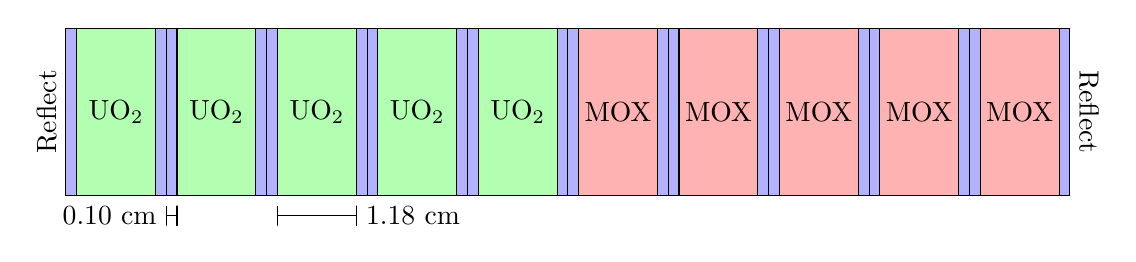
\begin{tikzpicture}[scale=0.85, every node/.style={scale=1}]
            \foreach \x in {0,1.5,...,6}
            \filldraw[xshift=\x cm, fill=green!30!white, draw=black]
            (0.160714286,0) rectangle (1.339285714,2.5) node[pos=.5] {UO$_2$};
            \foreach \x in {7.5,9,...,13.5}
            \filldraw[xshift=\x cm, fill=red!30!white, draw=black]
            (0.160714286,0) rectangle (1.339285714,2.5) node[pos=.5] {MOX};
            \foreach \x in {0,1.5,...,13.5}
            \filldraw[xshift=\x cm, fill=blue!30!white, draw=black] (0,0)
            rectangle (0.160714286,2.5);
            \foreach \x in {0,1.5,...,13.5}
            \filldraw[xshift=\x cm, fill=blue!30!white, draw=black]
            (1.339285714,0) rectangle (1.5,2.5);
            \draw[xshift=15cm,yshift=1.25cm] node[right]
            {\rotatebox{-90}{Reflect}};
            \draw[yshift=1.25cm] node[left] {\rotatebox{90}{Reflect}};
            \draw (1.5,-.15) -- (1.5,-.45) -- (1.5,-.30) node[left] {0.10 cm}
--
            (1.660714286,-.30) -- (1.660714286,-.15) -- (1.660714286, -.45);
            \draw (3.160714286,-.15) -- (3.160714286,-.45) --
(3.160714286,-.30)
            -- (4.339285714,-.30) node[right] {1.18 cm} -- (4.339285714,-.15)
            -- (4.339285714, -.45);
        \end{tikzpicture}
        \caption{Configuration for 10-pin Test Problem}
        \label{fig:10-pin_config}
    \end{figure*}

    Fuel pins were 1.08 cm thick with 0.09 cm of moderator on each side. The
    baseline pin-cell discretization consisted of 22 mesh cells of fuel
enclosed
    by three mesh cells of moderator on either side; therefore, each pin cell
    provided 28 energy-dependent snapshots.

    The second test case (adapted from \REF{Nichita1998}), more representative
of a     boiling water
    reactor (BWR), was comprised of seven assemblies each with 10 pins.  Three
    core configurations were used, and each core configuration had two unique
    assemblies.  Three fuel types were used, including 4.5\% enriched UO$_2$,
    2.5\% enriched UO$_2$, and 4.5\% enriched UO$_2$ with 5 wt\% Gd$_2$O$_3$.
    Core and assembly configurations are shown in Fig.~\ref{fig:BWRconfig}.
    Boundary conditions for this case were vacuum.

    \begin{figure*}[htb]
        \begin{minipage}[c]{\textwidth}
            \centering
            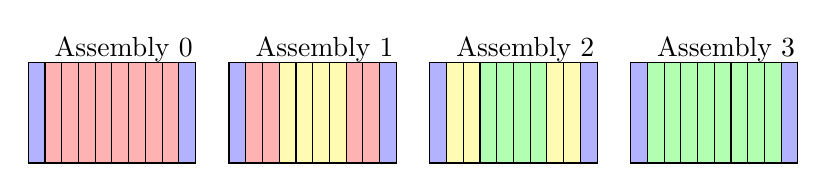
\begin{tikzpicture}[scale=0.85, every node/.style={scale=1}]
                \foreach \x in {0,2.25,3,5.25,6,8.25,9,11.25}
                \filldraw[xshift=\x cm,fill=blue!30!white,draw=black] (0,0)
                rectangle (0.25,1.5);
                \foreach \x in {.25,.5,.75,1,1.25,1.5,1.75,2,3.25,3.5,4.75,5}
                \filldraw[xshift=\x cm,fill=red!30!white,draw=black] (0,0)
                rectangle (0.25,1.5);
                \foreach \x in {3.75,4,4.25,4.5,6.25,6.5,7.75,8}
                \filldraw[xshift=\x cm,fill=yellow!30!white,draw=black] (0,0)
                rectangle (0.25,1.5);
                \foreach \x in
                {6.75,7,7.25,7.5,9.25,9.5,9.75,10,10.25,10.5,10.75,11}
                \filldraw[xshift=\x cm,fill=green!30!white,draw=black] (0,0)
                rectangle (0.25,1.5);
                \draw (0.25,1.7) node[right] {Assembly 0};%
                \draw (3.25,1.7) node[right] {Assembly 1};%
                \draw (6.25,1.7) node[right] {Assembly 2};%
                \draw (9.25,1.7) node[right] {Assembly 3};%
            \end{tikzpicture}
        \end{minipage}
        \begin{minipage}[c]{\textwidth}
            \centering
            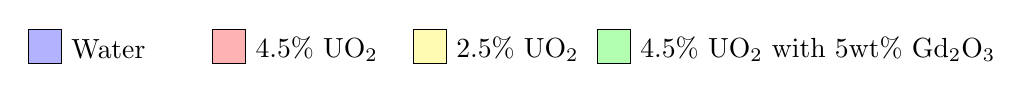
\begin{tikzpicture}[scale=0.85, every node/.style={scale=1}]
                \filldraw[xshift=-4cm,fill=blue!30!white,draw=black]
(-.25,-.25)
                rectangle (.25,.25) node[yshift=-.25cm, right] {Water};%
                \filldraw[xshift=-1.25cm,fill=red!30!white,draw=black]
                (-.25,-.25) rectangle (.25,.25) node[yshift=-.25cm, right]
                {4.5$\%$ UO$_2$};%
                \filldraw[xshift=1.75cm,fill=yellow!30!white,draw=black]
                (-.25,-.25) rectangle (.25,.25) node[yshift=-.25cm, right]
                {2.5$\%$ UO$_2$};%
                \filldraw[xshift=4.5cm,fill=green!30!white,draw=black]
                (-.25,-.25) rectangle (.25,.25) node[yshift=-.25cm, right]
                {4.5$\%$ UO$_2$ with 5wt$\%$ Gd$_2$O$_3$};%
            \end{tikzpicture}
        \end{minipage}
        \begin{minipage}[c]{\textwidth}
            \centering
            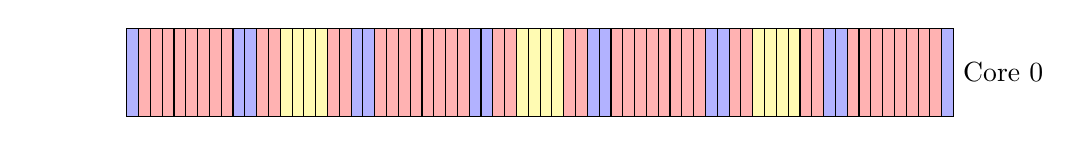
\begin{tikzpicture}[scale=1.5, every node/.style={scale=1}]
                \foreach \x in {0,.1,...,6.9}
                \filldraw[xshift=\x cm,fill=red!30!white,draw=black] (0,0)
                rectangle (0.1,.75);
                \foreach \x in {0,1,2,3,4,5,6,.9,1.9,2.9,3.9,4.9,5.9,6.9}
                \filldraw[xshift=\x cm,fill=blue!30!white,draw=black] (0,0)
                rectangle (0.1,.75);
                \foreach \x in {1.3,1.4,1.5,1.6,3.3,3.4,3.5,3.6,5.3,5.4,5.5,5.6}
                \filldraw[xshift=\x cm,fill=yellow!30!white,draw=black] (0,0)
                rectangle (0.1,.75);
                \draw (7,.375) node[right] {Core 0};%
                \draw (0,.375) node[left,color=white] {Core 0};
            \end{tikzpicture}
        \end{minipage}
        \begin{minipage}[c]{\textwidth}
            \centering
            \vspace*{.15cm}
            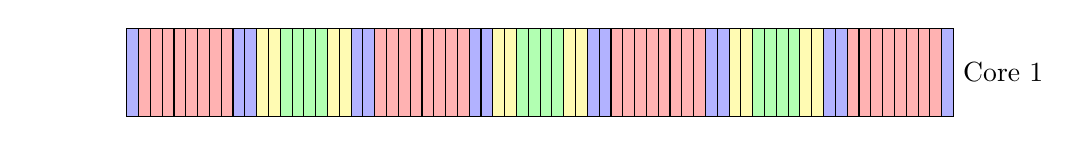
\begin{tikzpicture}[scale=1.5, every node/.style={scale=1}]
                \foreach \x in {0,.1,...,6.9}
                \filldraw[xshift=\x cm,fill=red!30!white,draw=black] (0,0)
                rectangle (0.1,.75);
                \foreach \x in {0,1,2,3,4,5,6,.9,1.9,2.9,3.9,4.9,5.9,6.9}
                \filldraw[xshift=\x cm,fill=blue!30!white,draw=black] (0,0)
                rectangle (0.1,.75);
                \foreach \x in {1.1,1.2,1.7,1.8,3.1,3.2,3.7,3.8,5.1,5.2,5.7,5.8}
                \filldraw[xshift=\x cm,fill=yellow!30!white,draw=black] (0,0)
                rectangle (0.1,.75);
                \foreach \x in {1.3,1.4,1.5,1.6,3.3,3.4,3.5,3.6,5.3,5.4,5.5,5.6}
                \filldraw[xshift=\x cm,fill=green!30!white,draw=black] (0,0)
                rectangle (0.1,.75);
                \draw (7,.375) node[right] {Core 1};%
                \draw (0,.375) node[left,color=white] {Core 1};
            \end{tikzpicture}
        \end{minipage}
        \begin{minipage}[c]{\textwidth}
            \centering
            \vspace*{.15cm}
            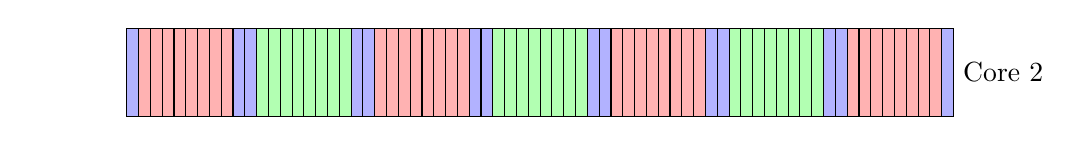
\begin{tikzpicture}[scale=1.5, every node/.style={scale=1}]
                \foreach \x in {0,.1,...,6.9}
                \filldraw[xshift=\x cm,fill=red!30!white,draw=black] (0,0)
                rectangle (0.1,.75);
                \foreach \x in {0,1,2,3,4,5,6,.9,1.9,2.9,3.9,4.9,5.9,6.9}
                \filldraw[xshift=\x cm,fill=blue!30!white,draw=black] (0,0)
                rectangle (0.1,.75);
                \foreach \x in {1.1,1.2,1.3,1.4,1.5,1.6,1.7,1.8,
                    3.1,3.2,3.3,3.4,3.5,3.6,3.7,3.8,
                    5.1,5.2,5.3,5.4,5.5,5.6,5.7,5.8}
                \filldraw[xshift=\x cm,fill=green!30!white,draw=black] (0,0)
                rectangle (0.1,.75);
                \draw (7,.375) node[right] {Core 2};%
                \draw (0,.375) node[left,color=white] {Core 2};
            \end{tikzpicture}
        \end{minipage}
        \caption{Configuration for BWR Test Problem}
        \label{fig:BWRconfig}
    \end{figure*}

    Fuel pins for the second problem were 0.72 cm thick with 0.27 cm of
    moderator on each side. Baseline pin-cell discretization consisted of 16
    mesh cells of fuel enclosed by six mesh cells of moderator; therefore, each
    pin cell provided 28 energy-dependent snapshots. With 70 pin cells, the
    total number of snapshots was 1960, but the right set of snapshots was
    identical to the left with respect to scalar flux.  For these
    simple problems, finer spatial and angular refinement was unnecessary.

    Because the test problem reference solution is a full transport
    approximation, boundary currents generally exhibit coupled angle-energy
    dependence.  By including snapshots that incorporate angular information,
    the resulting KLT basis may outperform snapshots based only on scalar flux
    $\phi$.  To include angular information, snapshots were taken of the
    energy-dependent partial current $J_{\text{left}}$.  Snapshots of the net
    current were previously considered, but those snapshots performed no better
    or worse than the partial current in all cases, so they are not presented
    here.  The direction selected for the partial current snapshots is
    arbitrary because the snapshot
    models were symmetric. Because step-characteristics discretization produces
    only one spatial unknown per cell, the snapshot generation approach used
    provided one ($\phi$) or two ($\phi$ and $J_{\text{left}}$) snapshots per
    spatial cell.

    In addition to inclusion of partial current snapshots for each test
    problem, the addition of snapshots of higher-order angular moments were
    studied.  These moments were generated by expanding the angular flux,
    $\psi$, through a Jacobi expansion in angle.  By this method the zeroth
    moment is equivalent to the partial current, while higher moments have less
    defined physical corollaries.  Inclusion of these moments (up to third
    order) was studied for both test problems and results are presented at the
    end of section \ref{sec:results}.

    \subsection{Generation of Snapshots for Test Problems}

    The goal for this work was to reduce the computational effort
    required to solve a problem, which is directly correlated with the success
    of a basis set, e.g. KLT.  Therefore, the proper selection of snapshots for
    KLT was a primary focus for this work.

    The first test problem was a 1-D approximation of the junction between a
    UO$_2$ and MOX assembly. Therefore, a number of small, representative
    subproblems are clear choices for snapshot generation. Models studied for
    this problem are summarized in Table \ref{tab:snapshots}. The simplest
    approach for generating snapshots is to model each pin cell individually,
    subject to reflecting boundary conditions on all surfaces, and to use
    snapshots (i.e., energy-dependent vectors in distinct spatial cells) from
    an individual pin cell or combine snapshots from both pin cell models.

    \begin{table*}[htb]
        \centering
        \caption{Summary of models used for snapshot generation for 10-pin test
            case}
        \begin{tabular}{c | l}\toprule
            Abbreviation    & Model to generate snapshots \\ \midrule
            MOX Pin         & MOX pin only \\
            UO$_2$ Pin      & UO$_2$ pin only \\
            Combined Pins   & Combined snapshots from UO$_2$ and MOX models,
and
            two-pin, UO$_2$-MOX model \\
            Full Assembly   & Repeating array of 10 UO$_2$ and 10 MOX pins \\
            \bottomrule
        \end{tabular}
        \label{tab:snapshots}
    \end{table*}

    A larger energy space is obtained if a single model includes more than one
    pin (fuel or moderator) in various arrangements.  For this work, an
    effectively $10\times 10$ (infinite lattice of ten UO$_2$ and ten MOX pins;
    denoted as the full assembly) was studied.  The full assembly model is the
    test problem of interest and should be expected to yield snapshots that
    represent the true multigroup solution with the lowest-order energy
    expansion.  Although other configurations were studied, configurations
    chosen for presentation provide a view into KLT using realistically
    attainable snapshots compared to the test problem.

    The second test problem was a 1-D approximation for a BWR core.  Models for
    this case are summarized in Table \ref{tab:bwrsnapshots}.  Three cases
    naturally arise from core construction: snapshots from the entire core
which
    are expected to perform the best, snapshots from the two unique assemblies
    used for each core configuration, and snapshots from each unique fuel pin
    used in the core configuration.

    \begin{table*}[htb]
        \centering
        \caption{Summary of models used for snapshot generation for BWR test
            case}
        \begin{tabular}{c | l}\toprule
            Abbreviation         & Model to generate snapshots \\ \midrule
            Full Core            & Snapshots from whole core model (i.e., the
            test problem) \\
            Combined Assemblies  & Snapshots from unique assemblies used in
core
            configuration \\
            Combined Pins        & Snapshots from unique pins used in core
            configuration \\
            \bottomrule
        \end{tabular}
        \label{tab:bwrsnapshots}
    \end{table*}

    \section{Results and Discussion}
    \label{sec:results}

    Typically, reactor analysis attempts to compute pin fission densities (or
    powers) with sub-$1\%$ errors.  To add an additional buffer, the goal of
    this work is to minimize the energy expansion order required to achieve
    sub-$0.1\%$ maximum relative fission density errors. The reference solution
    in all cases was a full multigroup response matrix solution for the given
    test problem with consistent angular expansion used throughout; in other
    words, any observed changes in the solution when using various energy bases
    was a function of only the energy basis.

    The reference solutions for the 10-pin problem for both energy group
    structures
    were compared.  The 44-group reference pin powers differ by a maximum
    of about $0.54\%$ compared to the 238-group reference pin powers.
    Since the goal is sub $0.1\%$ error, a low-order solution using the
    238-group basis outperforms a full-order expansion using the 44-group
    library.  However, this comparison is not quite fair as there are techniques
    to preserve the 44-group reaction rates, which may lead to a better
    44-group solution.

    With the exception of curves labeled by `DLP' and `mDLP', each curve in
    the plots to follow was generated using KLT
    basis with distinct snapshot data.
    The mDLP results represent the best case previously observed in
    \REF{Roberts2014}, which was to modify DLP with
    the average flux profile from the complete model.  Therefore, mDLP results
    are not entirely realistic because the solution
    for the test problem must be known {\it a priori}.

    Because the test problem and snapshot models studied were relatively small,
    timing studies would
    provide little insight.  However, for large 2-D or 3-D models (e.g.,
    assemblies or full cores), the snapshot
    models (e.g., pin cells or sub-assemblies) should be orders of magnitude
    less computationally expensive
    than the full model of interest.

    To improve computation time, databases that included responses for every
    order were created for each problem,
    allowing the relevant information to be read quickly.  Responses are a
    function of the $k$ eigenvalue; thus, a study into
    the number of $k$ values and range of $k$ values was explored.  Responses
    varied weakly with $k$; thus, databases with 8 $k$ values
    within a range of $\pm0.15$ of the solution eigenvalue provided results
that were indistinguishable from the non-database computations. This database
size allowed
    for third-order interpolation of responses.

    \subsection{10-pin Test Problem}

    As shown in Fig.~\ref{fig:10pin-44}, almost all KLT bases outperformed DLP
    for nearly all orders in the 10-pin problem while using the 44-group
    library.
    Snapshots generated by including UO$_2$ and MOX data perform as well as or
    better than mDLP, but single-pin
    models did not perform as well as mDLP.  However, mDLP was calculated using
    the solution, whereas the single-pin snapshot models were not.

    \begin{figure*}[tb]
        \centering
        \begin{subfigure}{0.5\textwidth}
            \centering
            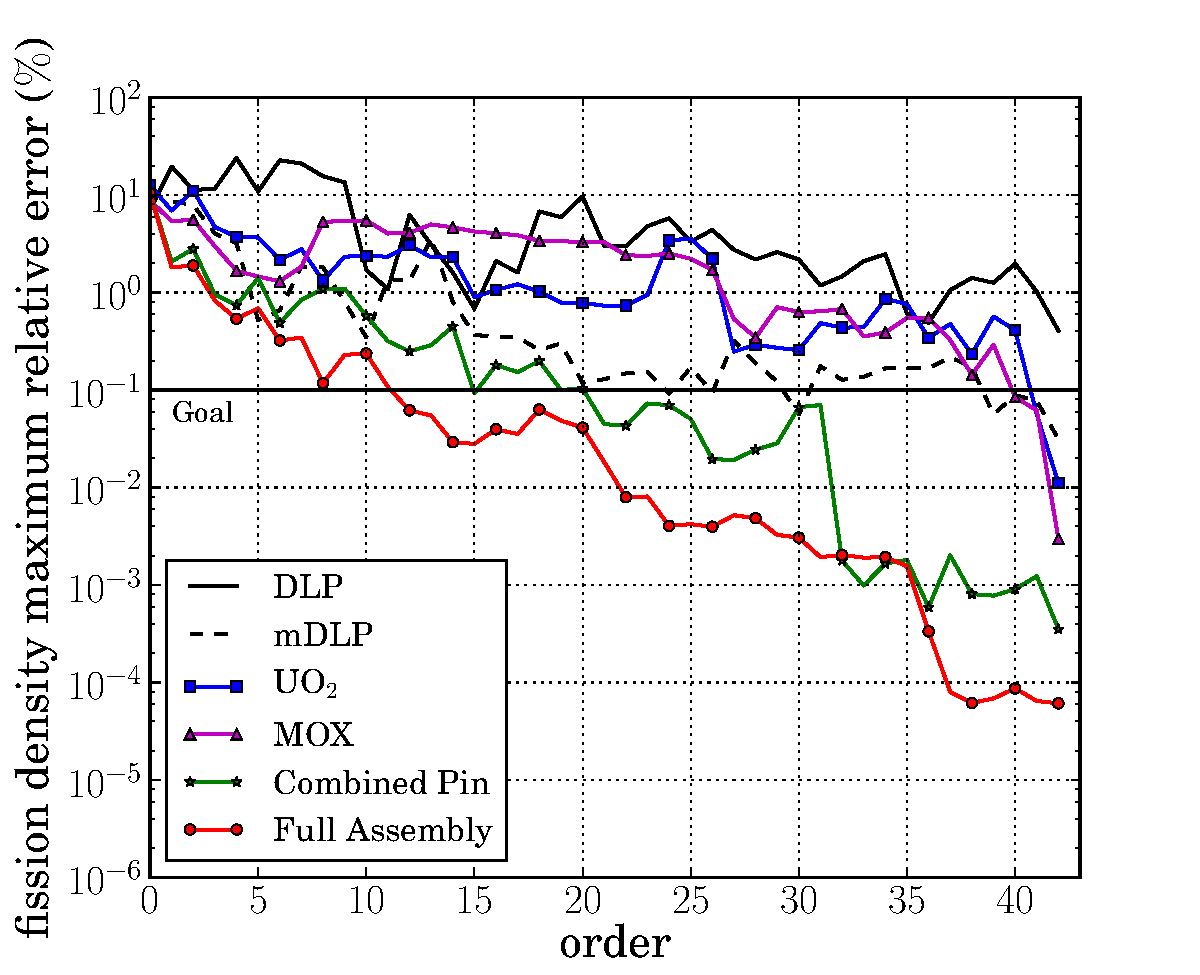
\includegraphics[trim=.1cm .25cm 2.0cm .4cm, clip=true,
            totalheight=0.261\textheight]
            {10pin_44_energy_basis_comparison_fission-44}
            \caption{Using only $\phi$ data}
            \label{fig:10pin-44a}
        \end{subfigure}%
        \begin{subfigure}{0.5\textwidth}
            \centering
            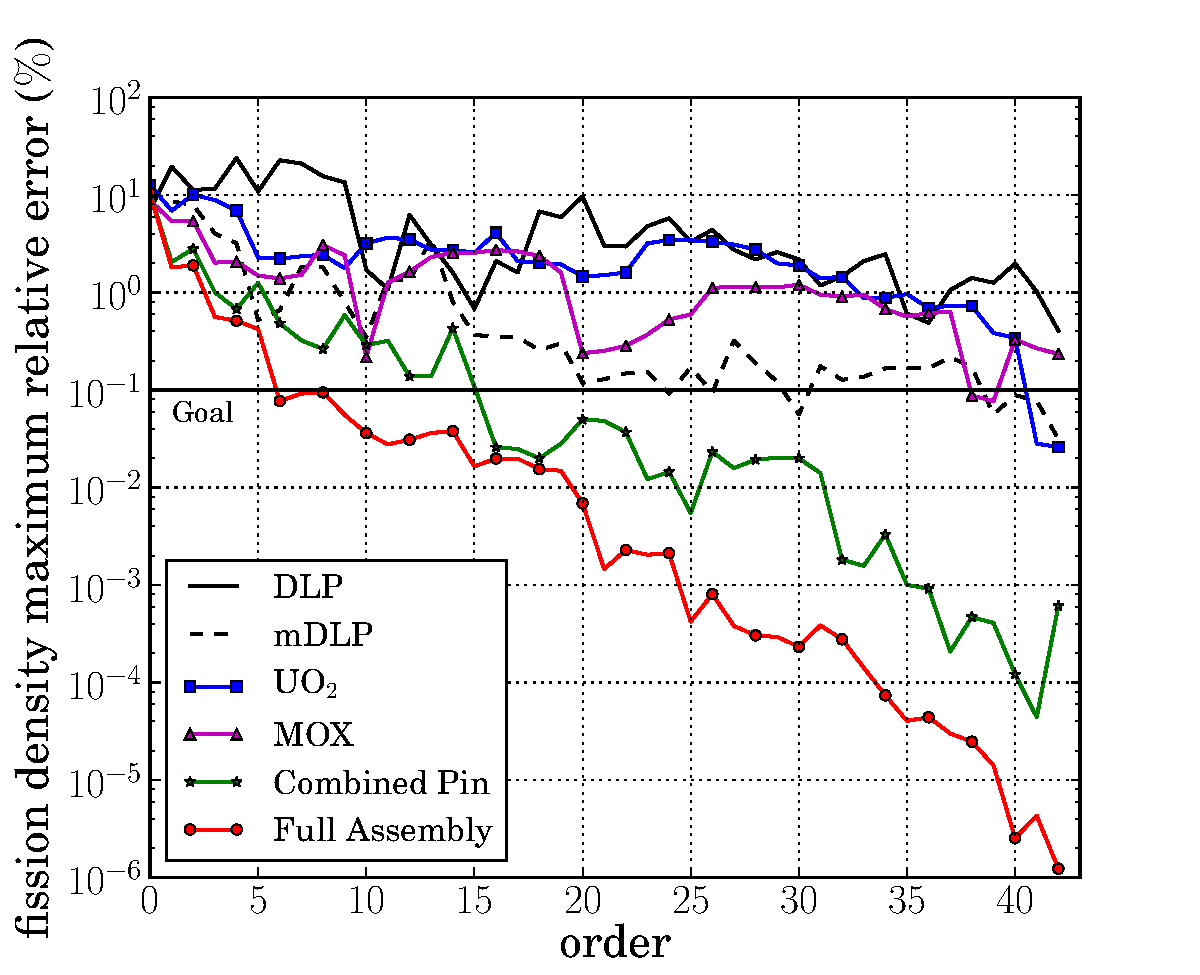
\includegraphics[trim=.1cm .25cm 2.0cm .4cm, clip=true,
            totalheight=0.261\textheight]
            {10pin_44_partial_energy_basis_comparison_fission-44}
            \caption{Using $\phi$ and $J_{\text{left}}$ data}
            \label{fig:10pin-44b}
        \end{subfigure}
        \caption{Relative error for 10-pin problem from 44-group library}
        \label{fig:10pin-44}
    \end{figure*}

    Fig.~\ref{fig:10pin-44a} shows results of using only the scalar flux $\phi$
    as data for snapshots.  When using snapshots from the full assembly model,
    the relative error fell below the 0.1$\%$ threshold at an energy order of
    approximately 12.  The combined-pin model required an energy expansion
order
    of at least 20, far from the goal of approximately five orders.

    When partial current snapshots were included with the scalar flux, results
    were
    improved, as shown in Fig.~\ref{fig:10pin-44b}. The full assembly snapshot
    model yielded sub-0.1$\%$ fission density errors with sixth-order
    expansions.  The combined-pin model required an energy expansion order of
    approximately 15.

    Results for the 238-group library were expected to be similar to the
    44-group results.  Figures presented from the 238-group library
    are shown only to 42nd energy order to facilitate comparison to the
44-group
    library.  With respect to the goal of order reduction, models should
    reach the 0.1$\%$ threshold by energy order of 44 regardless.

    Fig.~\ref{fig:10pin-238a} shows results of using only the scalar flux,
    $\phi$, as data for snapshots with the 238-group library.  When using
snapshots
    from the full assembly model, the relative error fell below the 0.1$\%$
    threshold at an energy order of approximately 14.
    The combined-pin model required an energy expansion order of at least 25.
    Low-order results from the 238-group library were similar to the 44-group
    results, specifically for the KLT basis models.

    \begin{figure*}[tb]
        \centering
        \begin{subfigure}{0.5\textwidth}
            \centering
            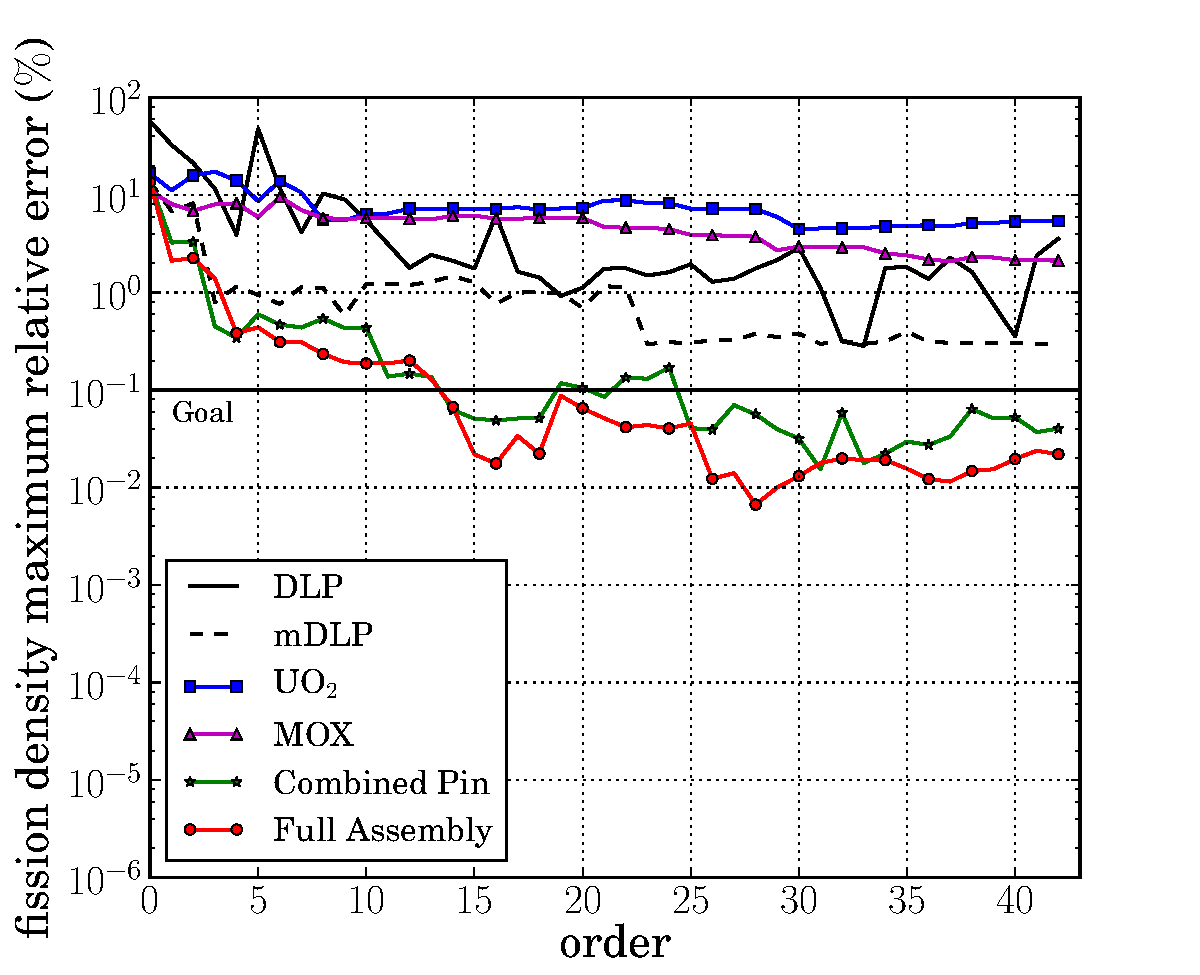
\includegraphics[trim=.1cm .25cm 2.0cm .4cm, clip=true,
            totalheight=0.261\textheight]
            {10pin_238_energy_basis_comparison_fission-44}
            \caption{Using only $\phi$ data}
            \label{fig:10pin-238a}
        \end{subfigure}%
        \begin{subfigure}{0.5\textwidth}
            \centering
            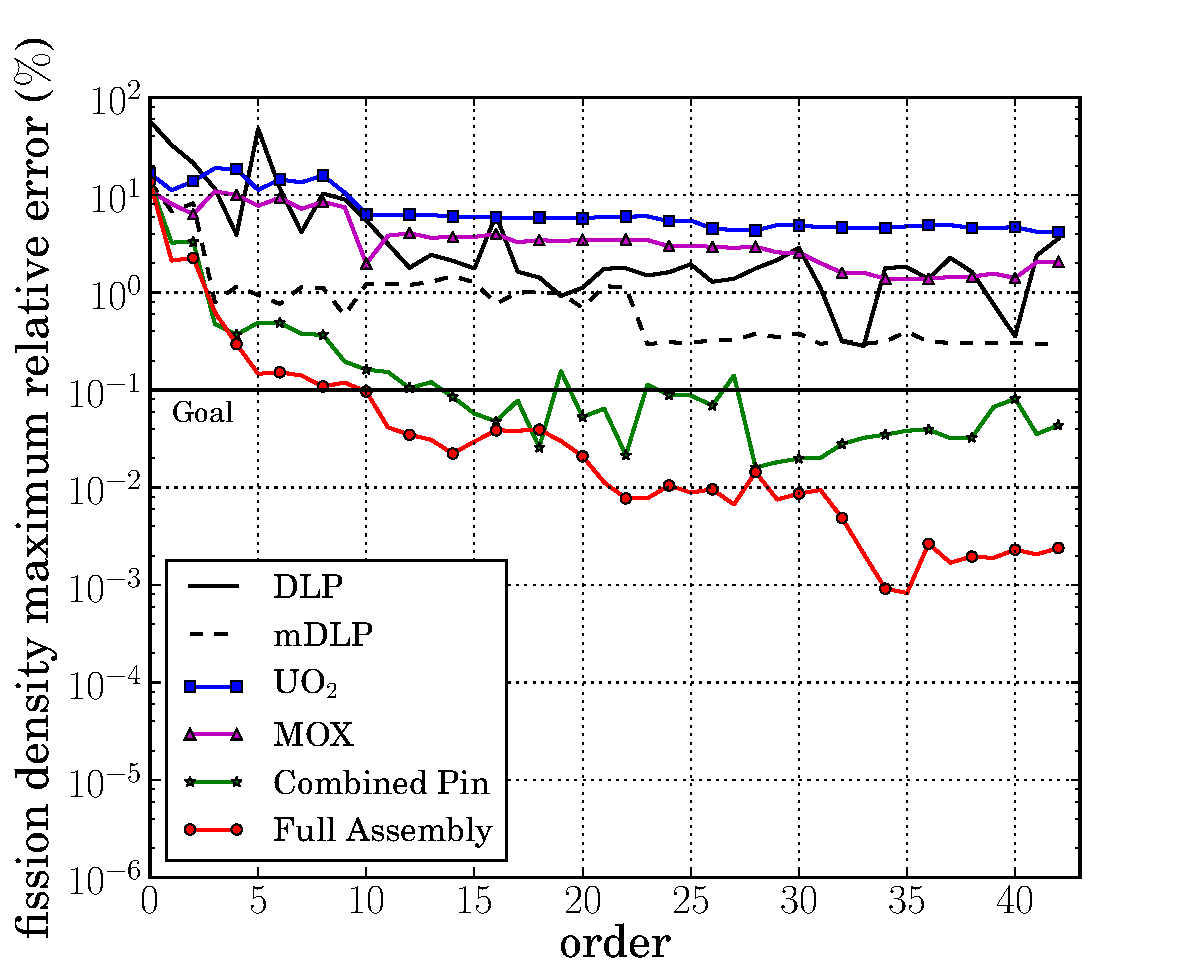
\includegraphics[trim=.1cm .25cm 2.0cm .4cm, clip=true,
            totalheight=0.261\textheight]
            {10pin_238_partial_energy_basis_comparison_fission-44}
            \caption{Using $\phi$ and $J_{\text{left}}$ data}
            \label{fig:10pin-238b}
        \end{subfigure}
        \caption{Relative error for 10-pin problem from 238-group library}
        \label{fig:10pin-238}
    \end{figure*}

    Results of including the partial current snapshots with the scalar flux
    snapshots are presented in Fig.\ref{fig:10pin-238b}.
    Inclusion of partial current snapshots contributed to the performance of
    each KLT model.
    In the best case (full assembly model), the relative error dropped below
    the 0.1$\%$ threshold at 10th order in energy, which was slightly improved
    from the 44-group results. The practical model (combined-pins) reaches the
    goal at an energy order of approximately 23.

    In 44-group and 238-group library tests, the combined-pin model performed
    reasonably well compared to the full assembly model.  The combined-pin
    model provided a practical option for expanding in energy.  The full
    assembly model required the solution {\it a priori}, while the
    combined-pins case utilized small problems to provide snapshots.  The
    single-pin
    models did not perform well because the models
    lacked physics information for one of the fuel types.

    Results from the inclusion of snapshots of the higher-order angular moments
    for the 10-pin test problem are shown in Fig.~\ref{fig:10-pin_angular}.
    The curves
    were created using snapshots from the full assembly model.  Results from
    the 44-group and 238-group libraries are shown side-by-side to ease
    comparison.  Adding the higher moments did not significantly affect the
    10-pin problem, consequently demonstrating that the relevant phase space
    information had already been captured. Therefore, curves for the higher
    moments were nearly equal to the zeroth moment curve.

    \begin{figure*}[tb]
        \centering
        \begin{subfigure}{0.5\textwidth}
            \centering
            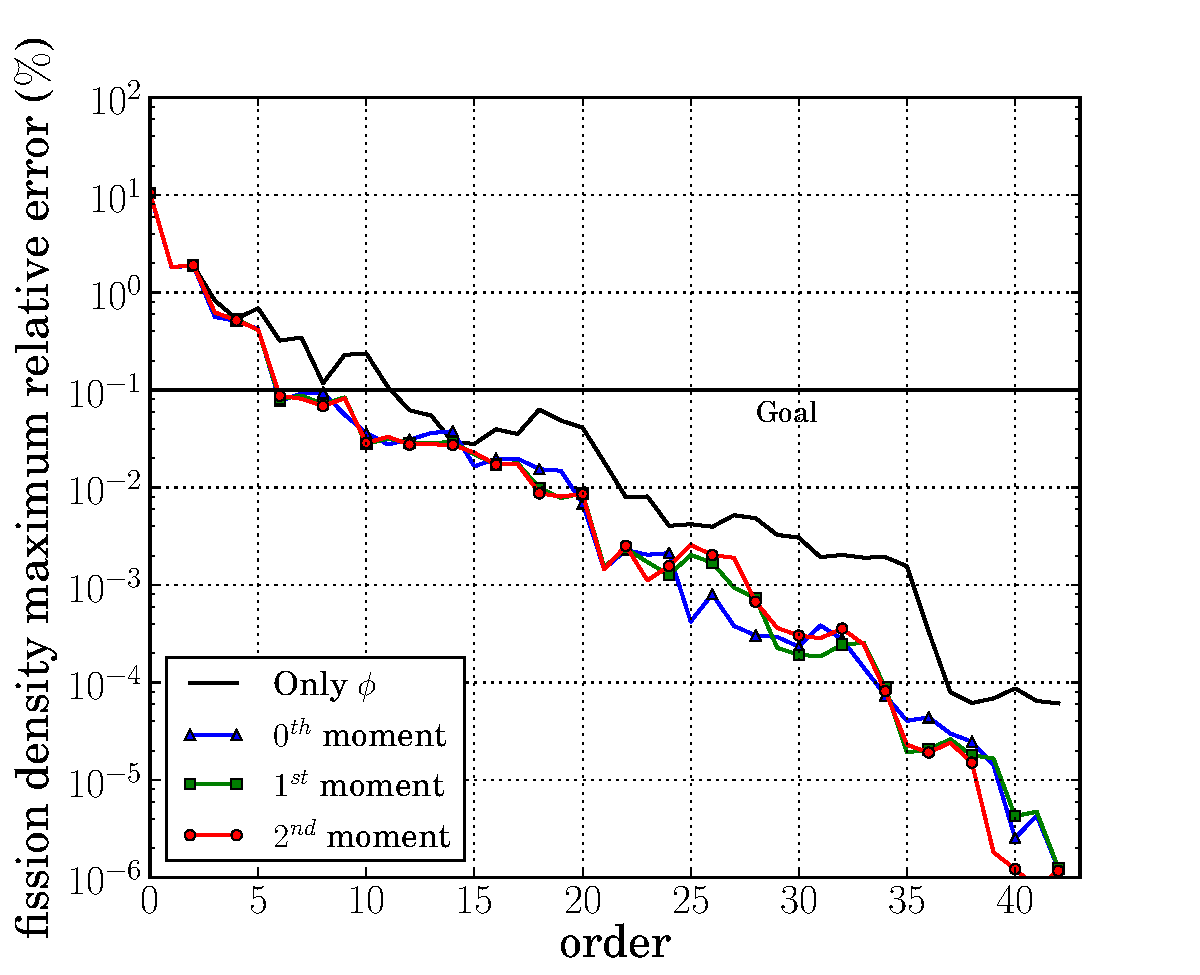
\includegraphics[trim=.1cm .25cm 2.0cm .4cm, clip=true,
            totalheight=0.261\textheight]
            {10pin_44_angular_comparison_fission_10-pin-44}
            \caption{From 44-group library}
            \label{fig:10-pin_angularA}
        \end{subfigure}%
        \begin{subfigure}{0.5\textwidth}
            \centering
            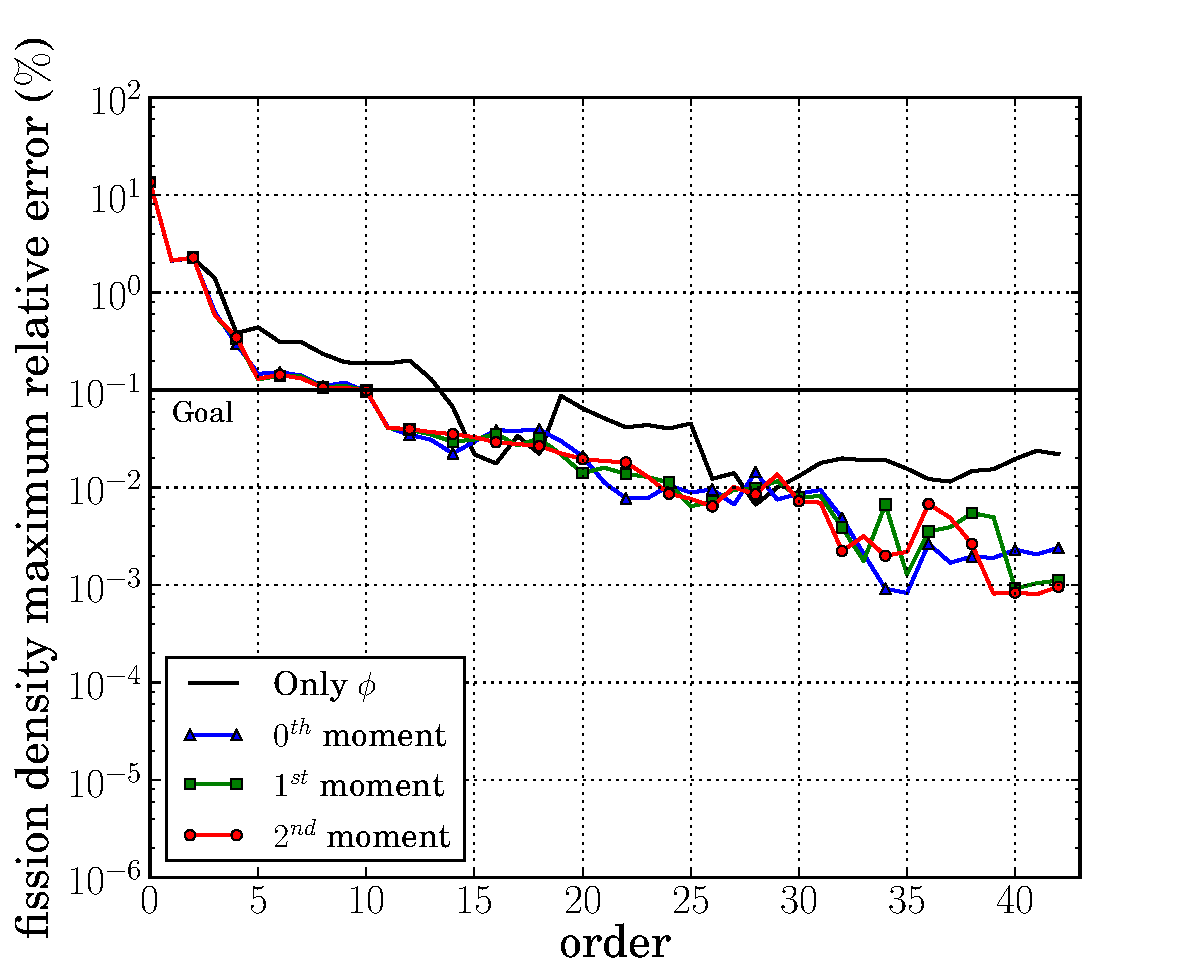
\includegraphics[trim=.1cm .25cm 2.0cm .4cm, clip=true,
            totalheight=0.261\textheight]
            {10pin_238_angular_comparison_fission_10-pin-44}
            \caption{From 238-group library}
            \label{fig:10-pin_angularB}
        \end{subfigure}
        \caption{Relative error for 10-pin problem using higher-order moment
            data}
        \label{fig:10-pin_angular}
    \end{figure*}

    \subsection{BWR Test Problem}

    In this section, the methods described
    were applied to the BWR test problem. For the BWR test problem, each core
configuration was increasingly
    inhomogeneous, and thus, more difficult to model.  The difficulty
    manifests in a larger error for the same energy order while progressing
    through configurations.

    Figures for this section are shown as side-by-side comparisons of using
    snapshots of only $\phi$ versus using snapshots including $\phi$ and the
    leftward partial current for basis generation. Three core configurations
    were explored, as shown.
    For the best case (using snapshots from the core model) using the 44-group
    library, Configuration 0,
    shown in Fig.~\ref{fig:core0-44}, required approximately six orders when
    using only scalar flux, and approximately five orders when including partial
    current to reach the target accuracy. Configuration 1, shown in Fig.
    \ref{fig:core1-44}, required seven
    and eight orders, respectively, for using only $\phi$ snapshots and
    including partial
    current snapshots. Finally, Configuration 2, shown in Fig.
    \ref{fig:core2-44},
    required 13 and 11 orders, respectively, to achieve the goal of sub-$0.1\%$
    maximum relative fission density errors.  The increasing inhomogeneity
leads to expansions requiring more energy degrees of freedom to achieve
the
    same relative error.

    \begin{figure*}[tb]
        \centering
        \begin{subfigure}{0.5\textwidth}
            \centering
            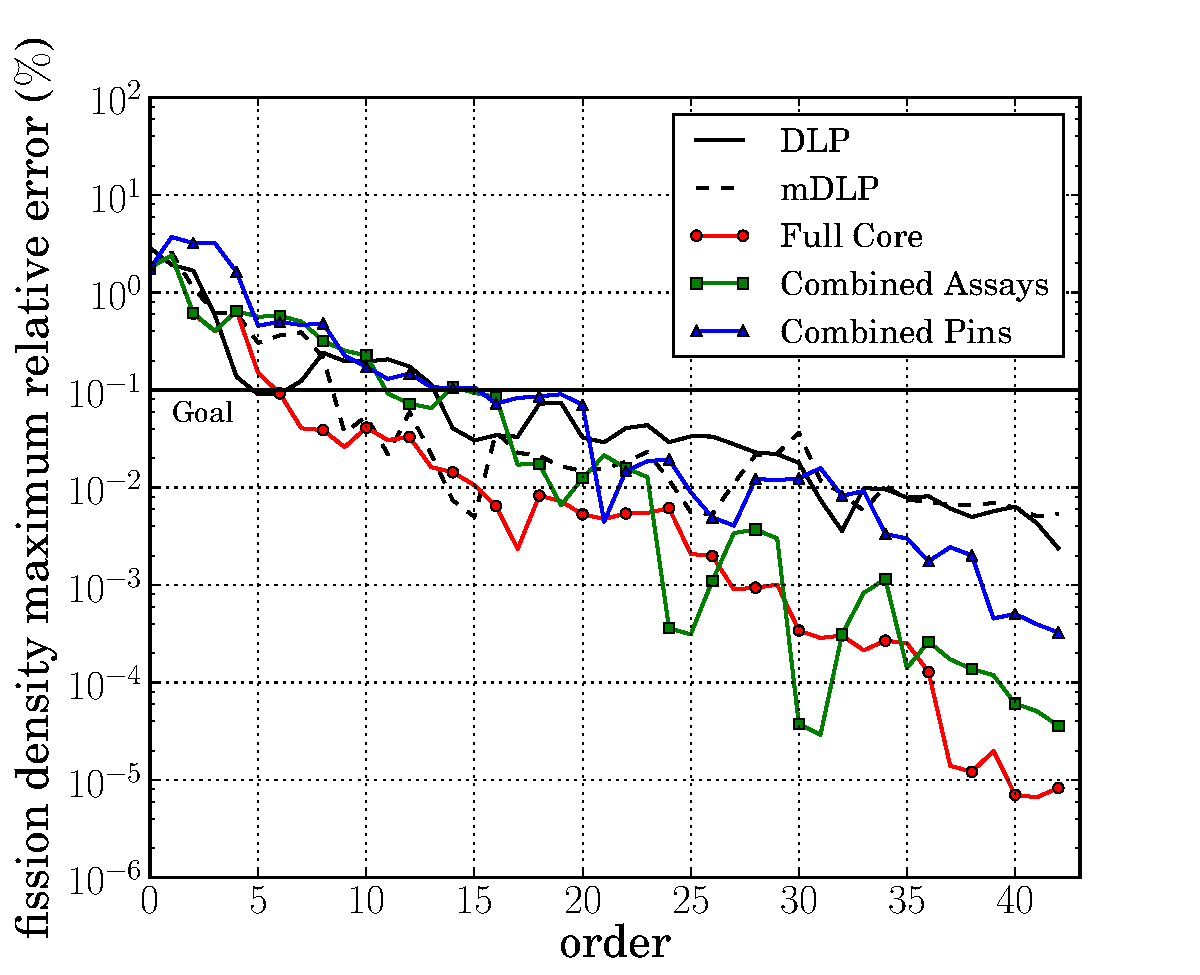
\includegraphics[trim=.1cm .25cm 2.0cm .4cm, clip=true,
            totalheight=0.261\textheight]
            {BWR0_44_energy_basis_comparison_fission-44}
            \caption{Using only $\phi$ data}
            \label{fig:core0-44a}
        \end{subfigure}%
        \begin{subfigure}{0.5\textwidth}
            \centering
            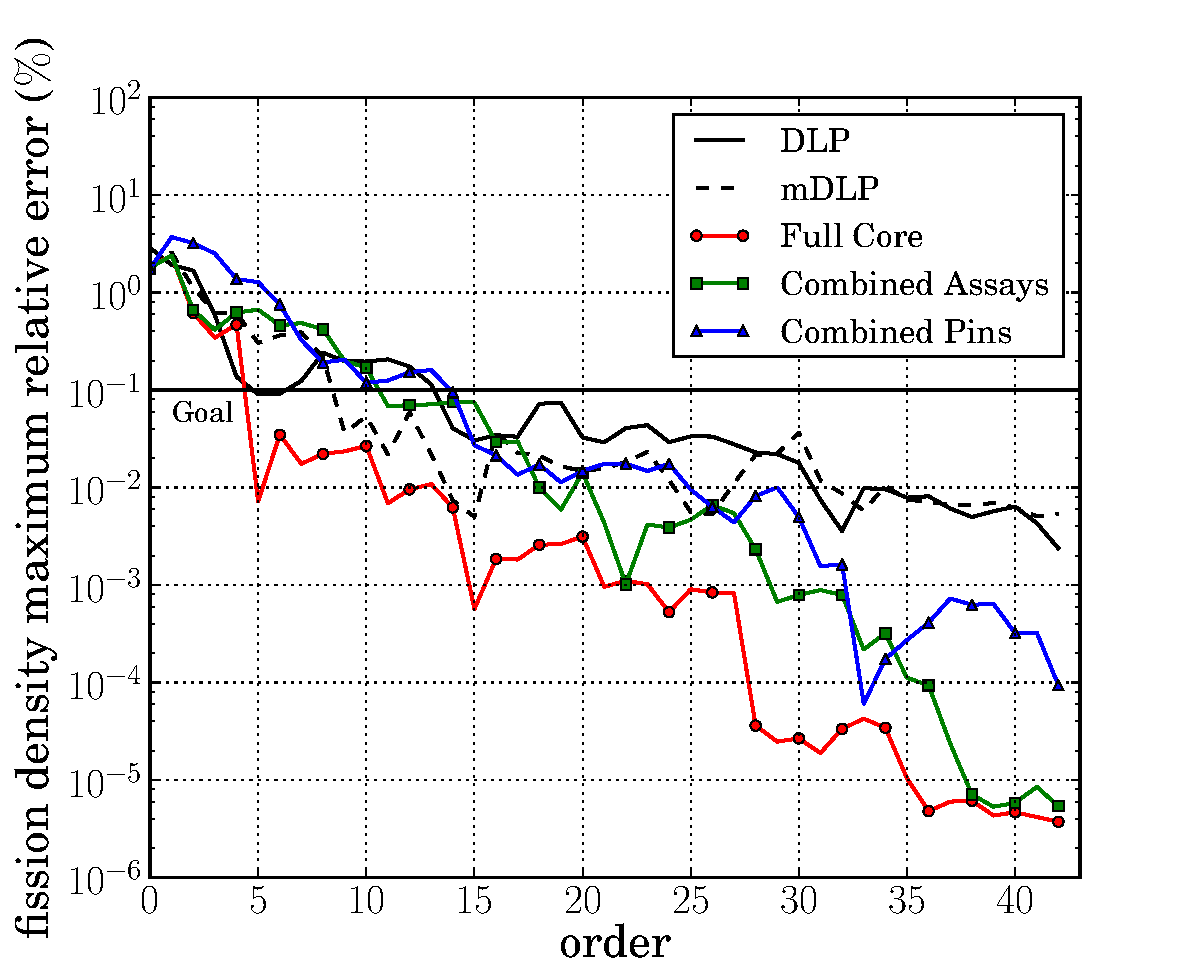
\includegraphics[trim=.1cm .25cm 2.0cm .4cm, clip=true,
            totalheight=0.261\textheight]
            {BWR0_44_partial_energy_basis_comparison_fission-44}
            \captionof{figure}{Using $\phi$ and $J_{\text{left}}$ data}
            \label{fig:core0-44b}
        \end{subfigure}
        \caption{Relative error for BWR test problem, Configuration 0, from
            44-group library}
        \label{fig:core0-44}
    \end{figure*}

    \begin{figure*}[tb]
        \centering
        \begin{subfigure}{0.5\textwidth}
            \centering
            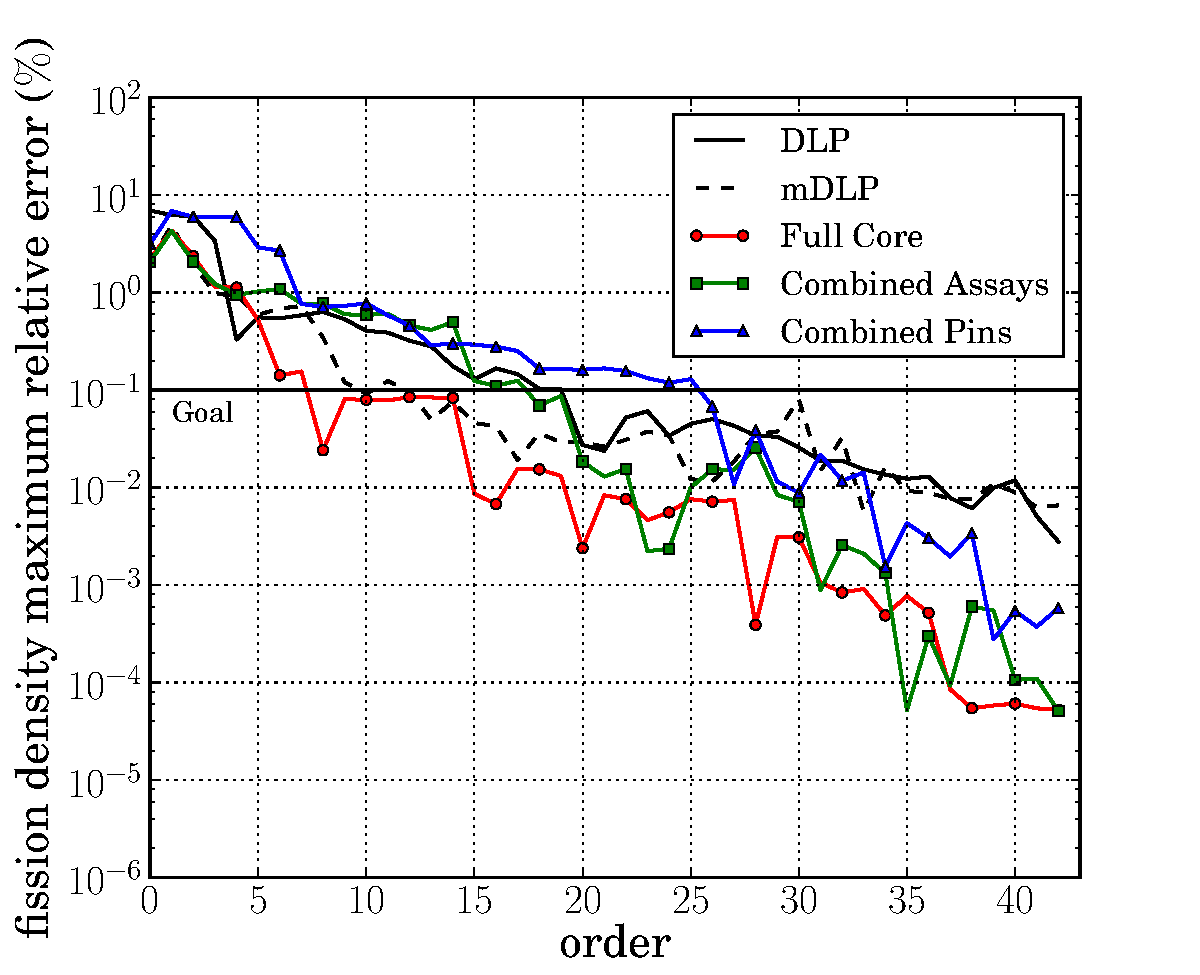
\includegraphics[trim=.1cm .25cm 2.0cm .4cm, clip=true,
            totalheight=0.261\textheight]
            {BWR1_44_energy_basis_comparison_fission-44}
            \caption{Using only $\phi$ data}
            \label{fig:core1-44a}
        \end{subfigure}%
        \begin{subfigure}{0.5\textwidth}
            \centering
            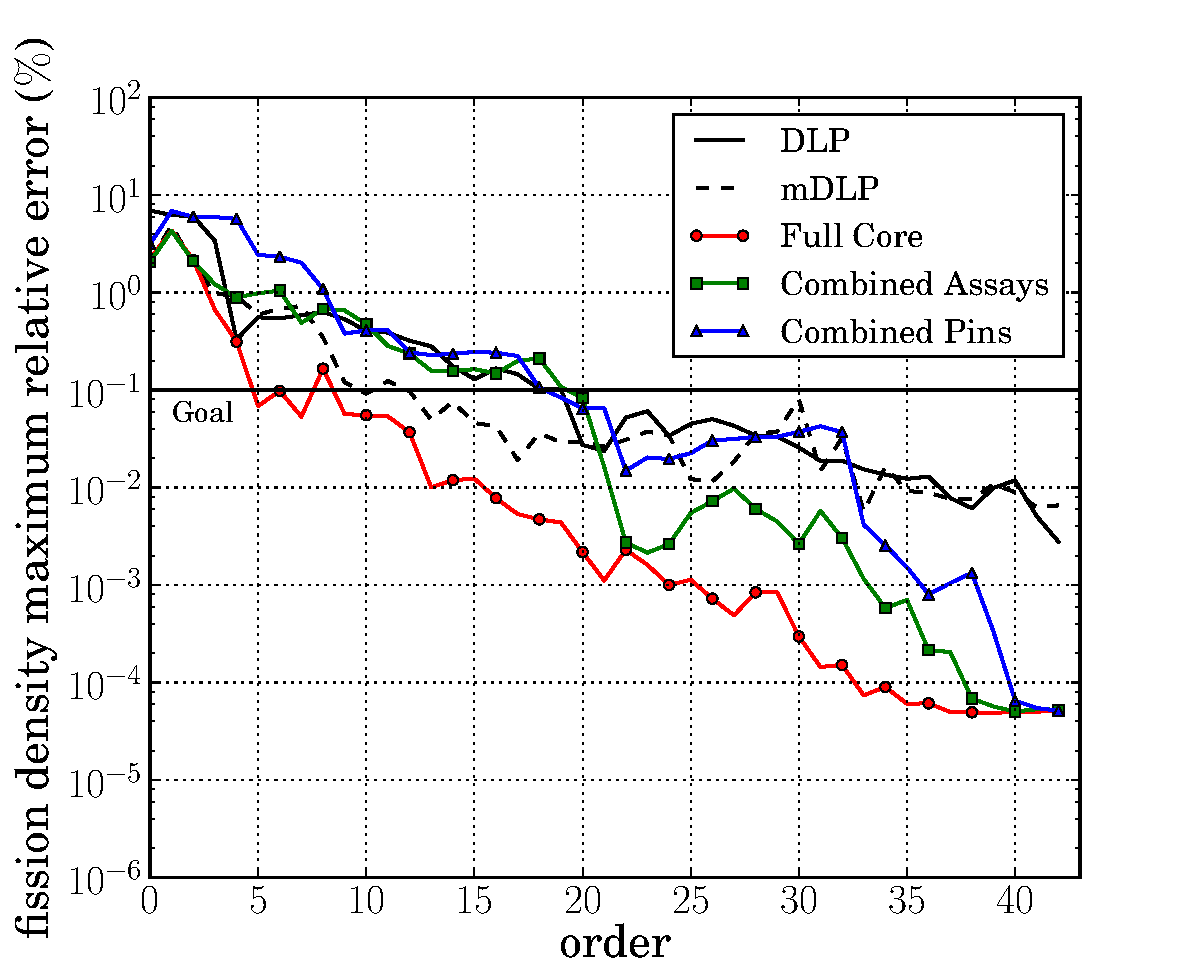
\includegraphics[trim=.1cm .25cm 2.0cm .4cm, clip=true,
            totalheight=0.261\textheight]
            {BWR1_44_partial_energy_basis_comparison_fission-44}
            \captionof{figure}{Using $\phi$ and $J_{\text{left}}$ data}
            \label{fig:core1-44b}
        \end{subfigure}
        \caption{Relative error for BWR test problem, Configuration 1, from
            44-group library}
        \label{fig:core1-44}
    \end{figure*}

    \begin{figure*}[tb]
        \centering
        \begin{subfigure}{0.5\textwidth}
            \centering
            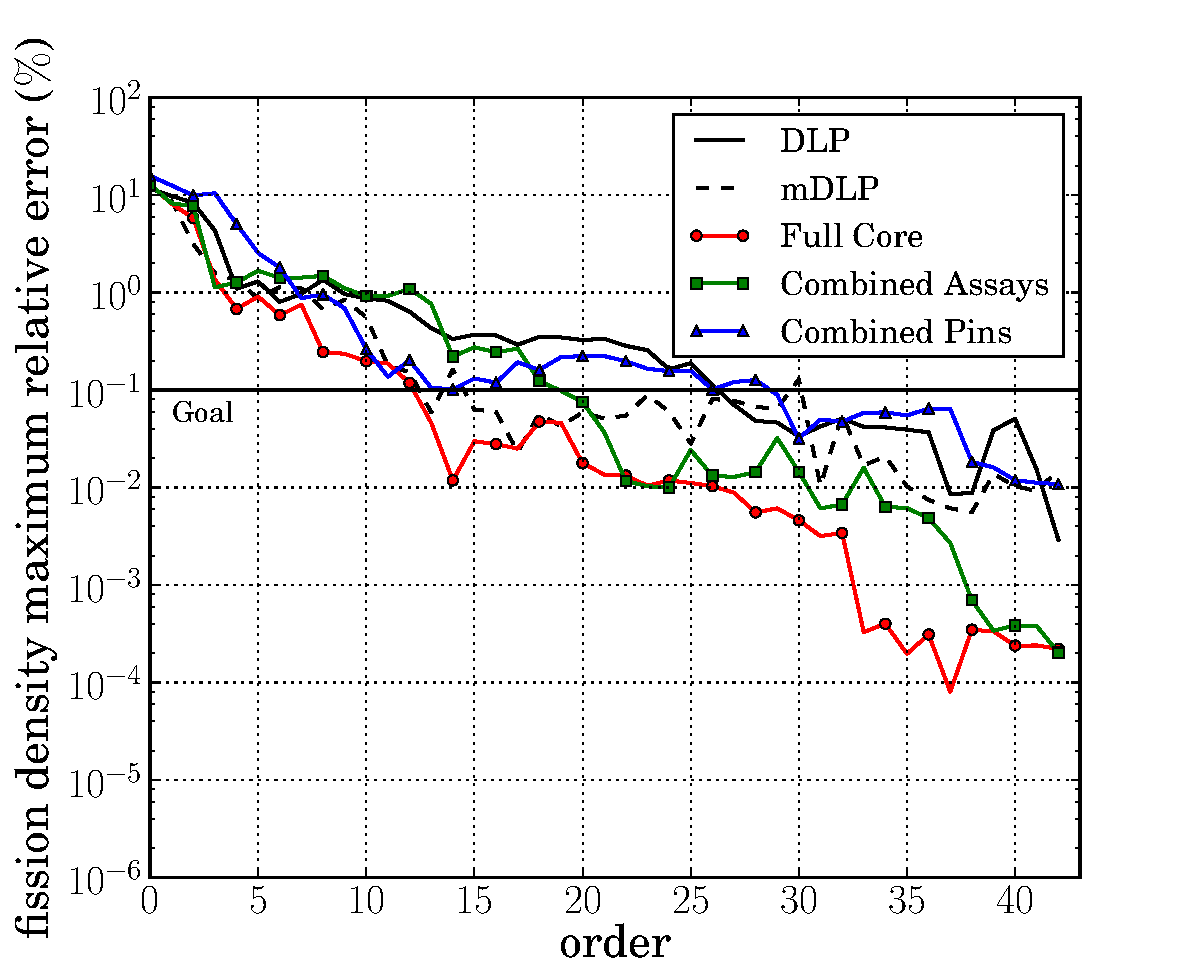
\includegraphics[trim=.1cm .25cm 2.0cm .4cm, clip=true,
            totalheight=0.261\textheight]
            {BWR2_44_energy_basis_comparison_fission-44}
            \caption{Using only $\phi$ data}
            \label{fig:core2-44a}
        \end{subfigure}%
        \begin{subfigure}{0.5\textwidth}
            \centering
            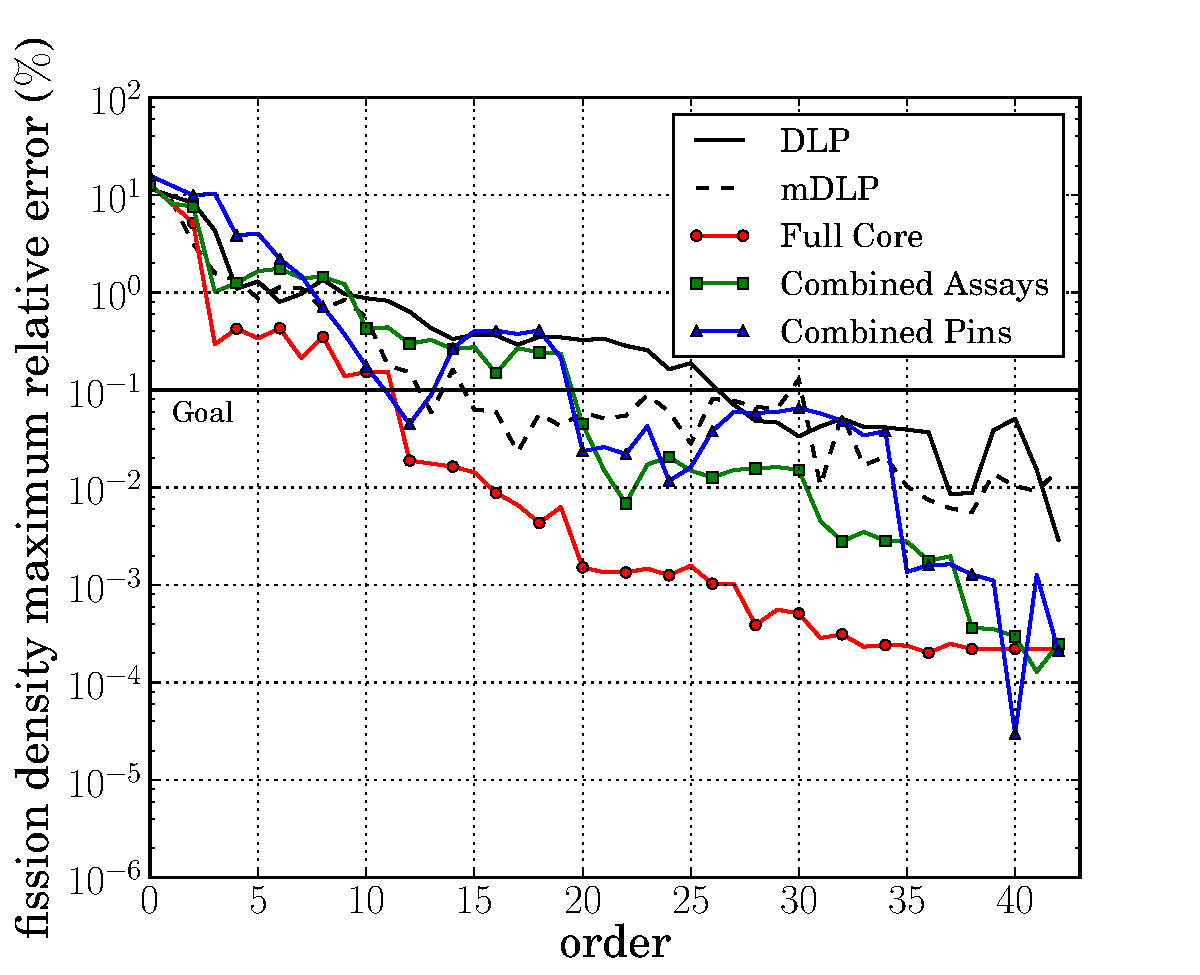
\includegraphics[trim=.1cm .25cm 2.0cm .4cm, clip=true,
            totalheight=0.261\textheight]
            {BWR2_44_partial_energy_basis_comparison_fission-44}
            \captionof{figure}{Using $\phi$ and $J_{\text{left}}$ data}
            \label{fig:core2-44b}
        \end{subfigure}
        \caption{Relative error for BWR test problem, Configuration 2, from
            44-group library}
        \label{fig:core2-44}
    \end{figure*}

    The practical, combined-pins and combined-assemblies, models required
    energy orders of approximately 15 and 14 to reach the target accuracy when
using
    only scalar flux snapshots and using both scalar flux and partial
    current snapshots, respectively, for Configuration 0. In Configuration
    1, these models required at
    least order 20 to reach the goal while including snapshots of only the
    scalar flux. Including snapshots of the
    partial current reduced the required order to 19. Finally, Configuration
    2 required approximately equivalent orders as Configuration 1 for
    practical models.

    The only configuration that met the second goal of an order of magnitude
    reduction in required energy order was configuration 0, and
    only for the unpractical case of the full core model. For
    the BWR test problem, mDLP performed much better than for the 10-pin test
    problem. However,the full core solution was used to
    generate the shape function for the modified polynomials, which should lead
    to the best possible, but not a practical, performance of mDLP.
    For each core configuration, the combined-pins and combined-assemblies
    models performed similarly, but the combined-assemblies model was
    superior. However, the performance of the combined-pins model was
    strong considering the simplicity of the snapshot model.

    Analysis for the BWR test problem was repeated using the 238-group
    library. For
    this case, Configuration 0, shown in Fig.~\ref{fig:core0-238}, required
    orders of 11 and 4, respectively, for using snapshots of only $\phi$ and
    including partial
    current snapshots. Configuration 1, shown in Fig.~\ref{fig:core1-238},
    required
    orders of 12 and 9, respectively. Configuration 2, shown in Fig.
    \ref{fig:core2-238}, required 22 and 10, respectively, to meet the first
    goal of sub-$0.1\%$ errors in the fission density.

    \begin{figure*}[tb]
        \centering
        \begin{subfigure}{0.5\textwidth}
            \centering
            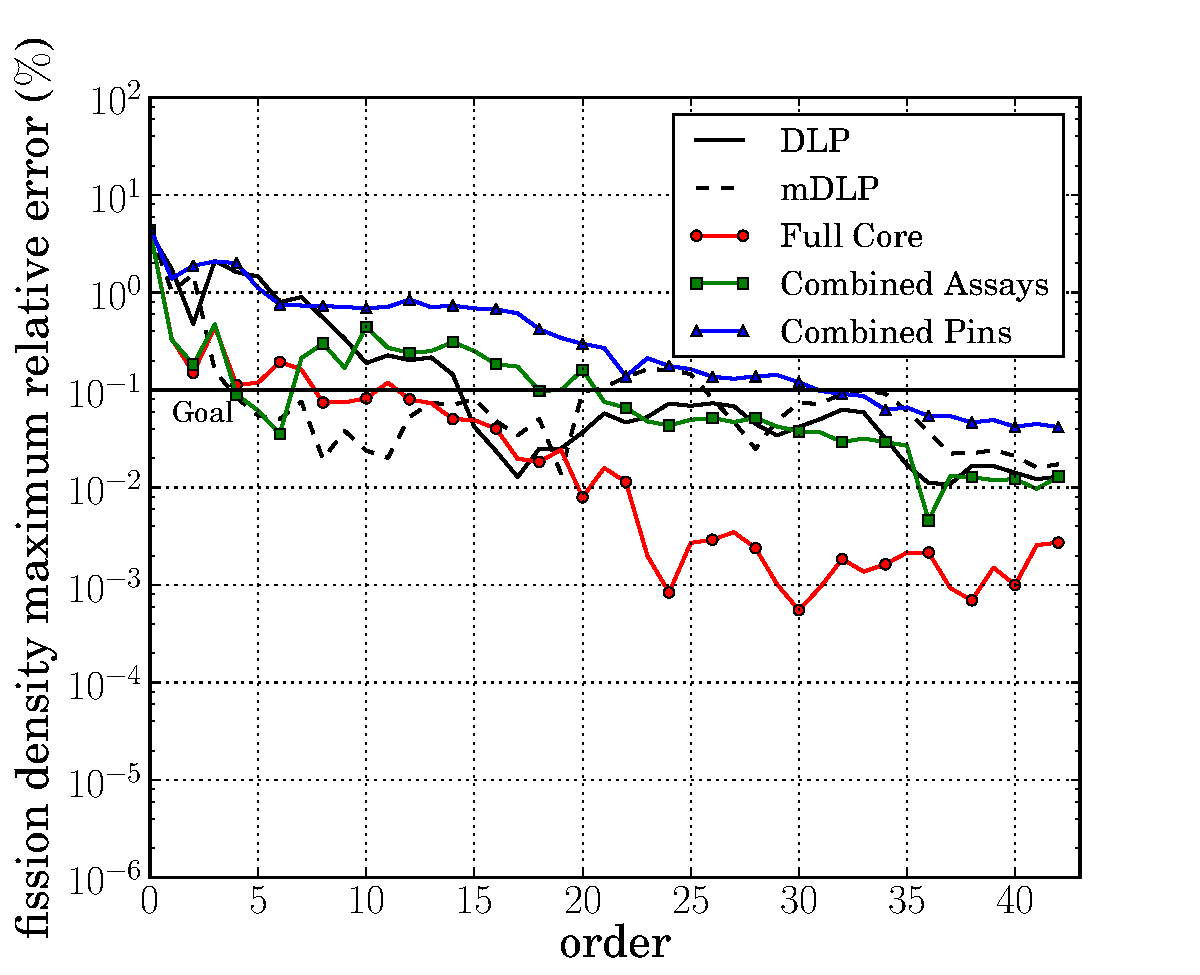
\includegraphics[trim=.1cm .25cm 2.0cm .4cm, clip=true,
            totalheight=0.261\textheight]
            {BWR0_238_energy_basis_comparison_fission-44}
            \caption{Using only $\phi$ data}
            \label{fig:core0-238a}
        \end{subfigure}%
        \begin{subfigure}{0.5\textwidth}
            \centering
            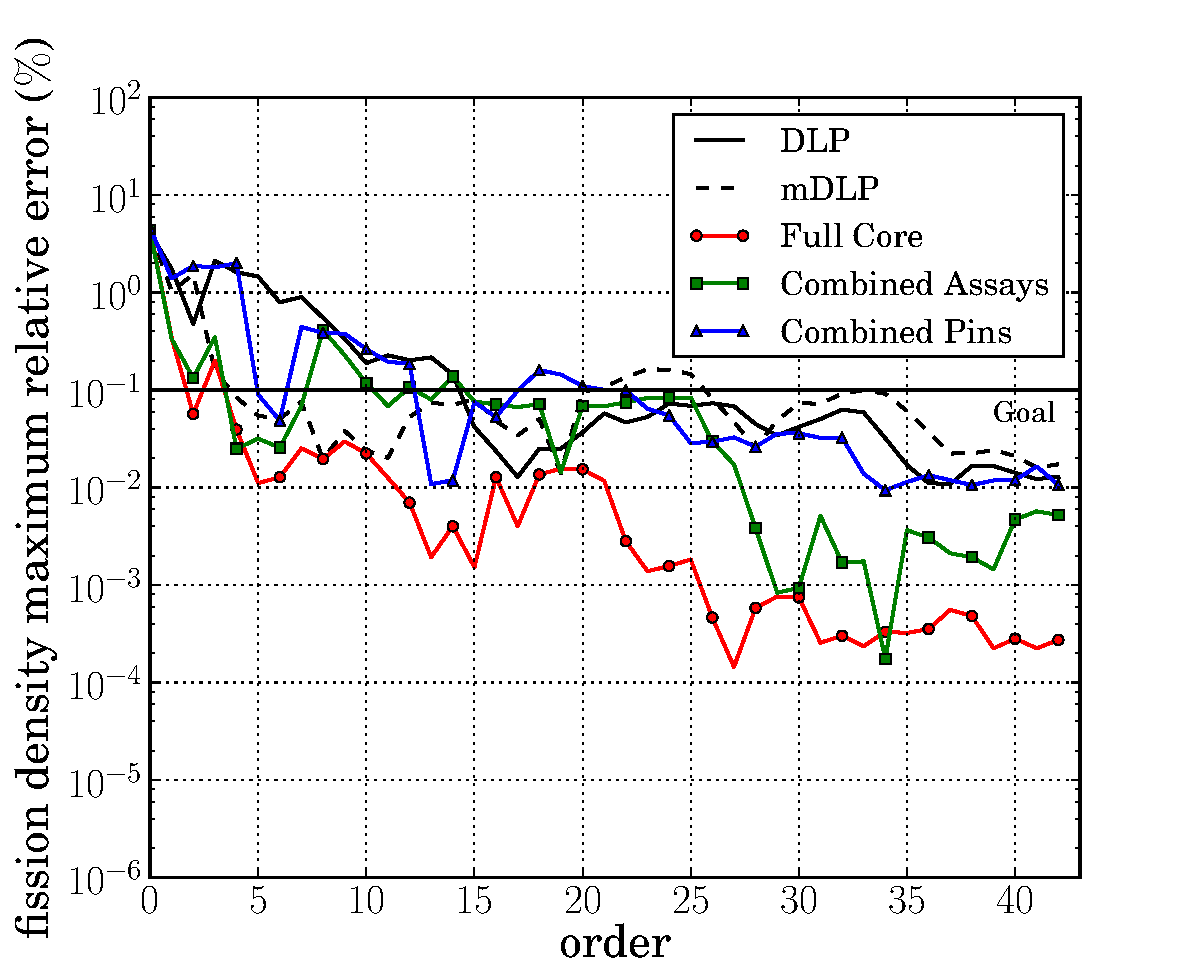
\includegraphics[trim=.1cm .25cm 2.0cm .4cm, clip=true,
            totalheight=0.261\textheight]
            {BWR0_238_partial_energy_basis_comparison_fission-44}
            \captionof{figure}{Using $\phi$ and $J_{\text{left}}$ data}
            \label{fig:core0-238b}
        \end{subfigure}
        \caption{Relative error for BWR test problem, Configuration 0, from
            238-group library}
        \label{fig:core0-238}
    \end{figure*}

    \begin{figure*}[tb]
        \centering
        \begin{subfigure}{0.5\textwidth}
            \centering
            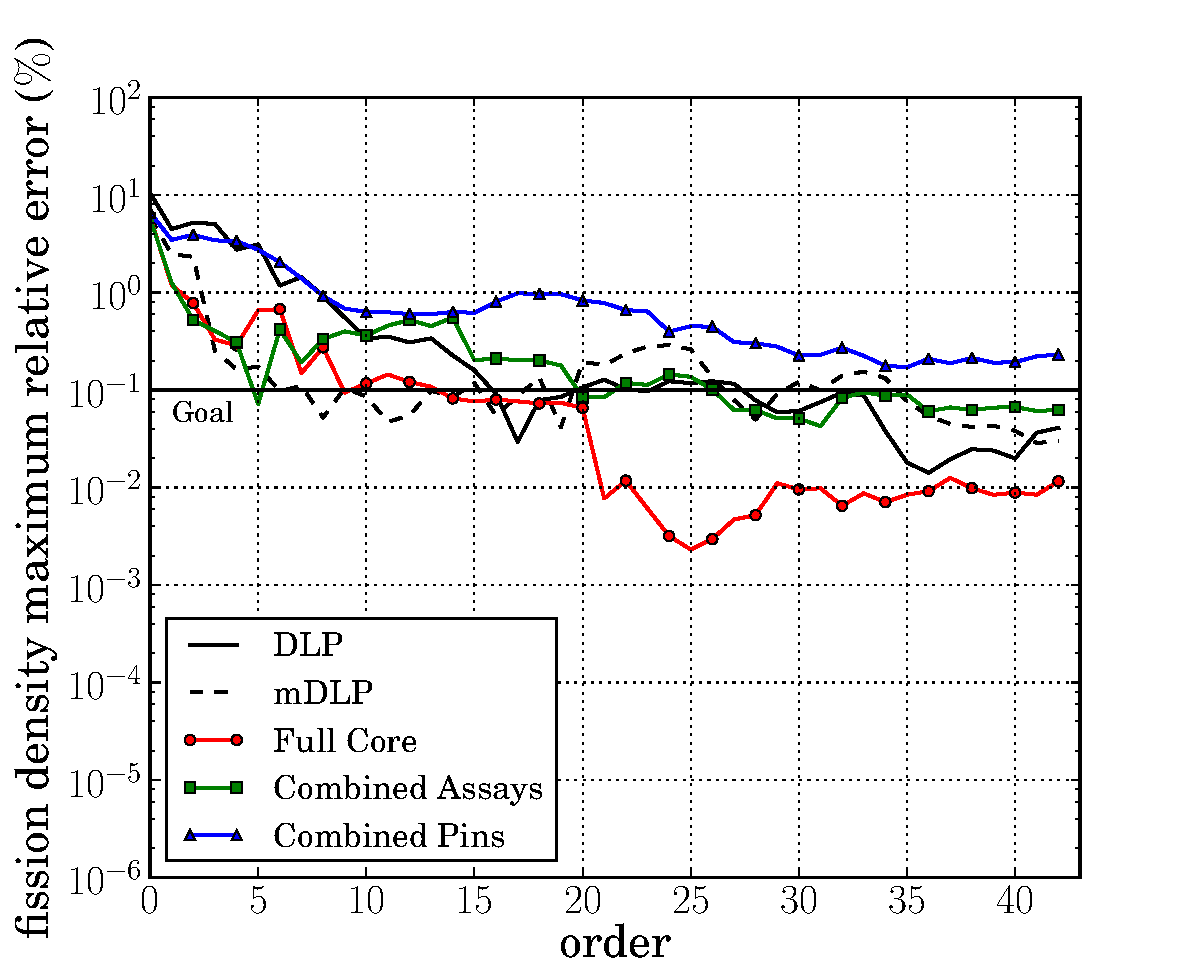
\includegraphics[trim=.1cm .25cm 2.0cm .4cm, clip=true,
            totalheight=0.261\textheight]
            {BWR1_238_energy_basis_comparison_fission-44}
            \caption{Using only $\phi$ data}
            \label{fig:core1-238a}
        \end{subfigure}%
        \begin{subfigure}{0.5\textwidth}
            \centering
            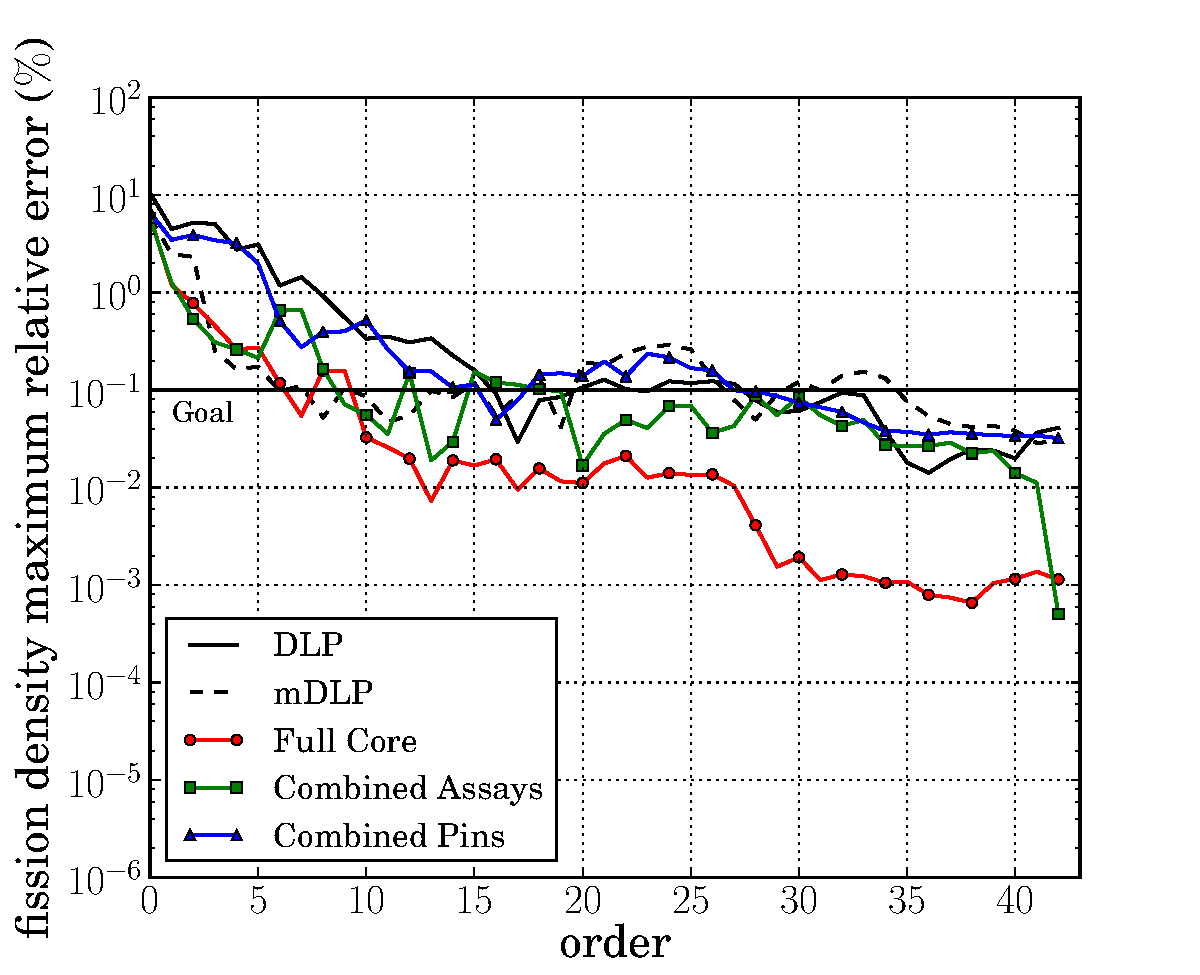
\includegraphics[trim=.1cm .25cm 2.0cm .4cm, clip=true,
            totalheight=0.261\textheight]
            {BWR1_238_partial_energy_basis_comparison_fission-44}
            \captionof{figure}{Using $\phi$ and $J_{\text{left}}$ data}
            \label{fig:core1-238b}
        \end{subfigure}
        \caption{Relative error for BWR test problem, Configuration 1, from
            238-group library}
        \label{fig:core1-238}
    \end{figure*}

    \begin{figure*}[tb]
        \centering
        \begin{subfigure}{0.5\textwidth}
            \centering
            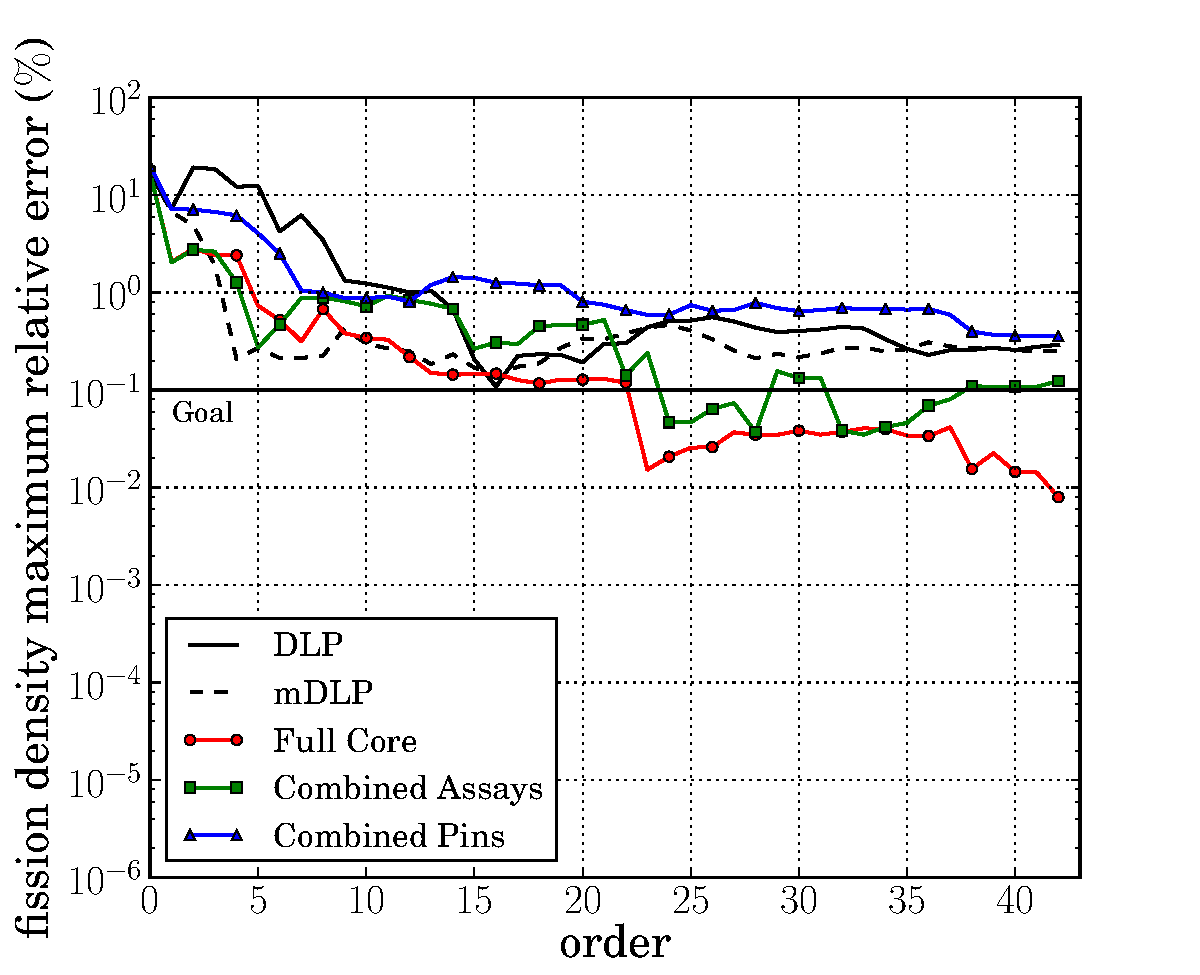
\includegraphics[trim=.1cm .25cm 2.0cm .4cm, clip=true,
            totalheight=0.261\textheight]
            {BWR2_238_energy_basis_comparison_fission-44}
            \caption{Using only $\phi$ data}
            \label{fig:core2-238a}
        \end{subfigure}%
        \begin{subfigure}{0.5\textwidth}
            \centering
            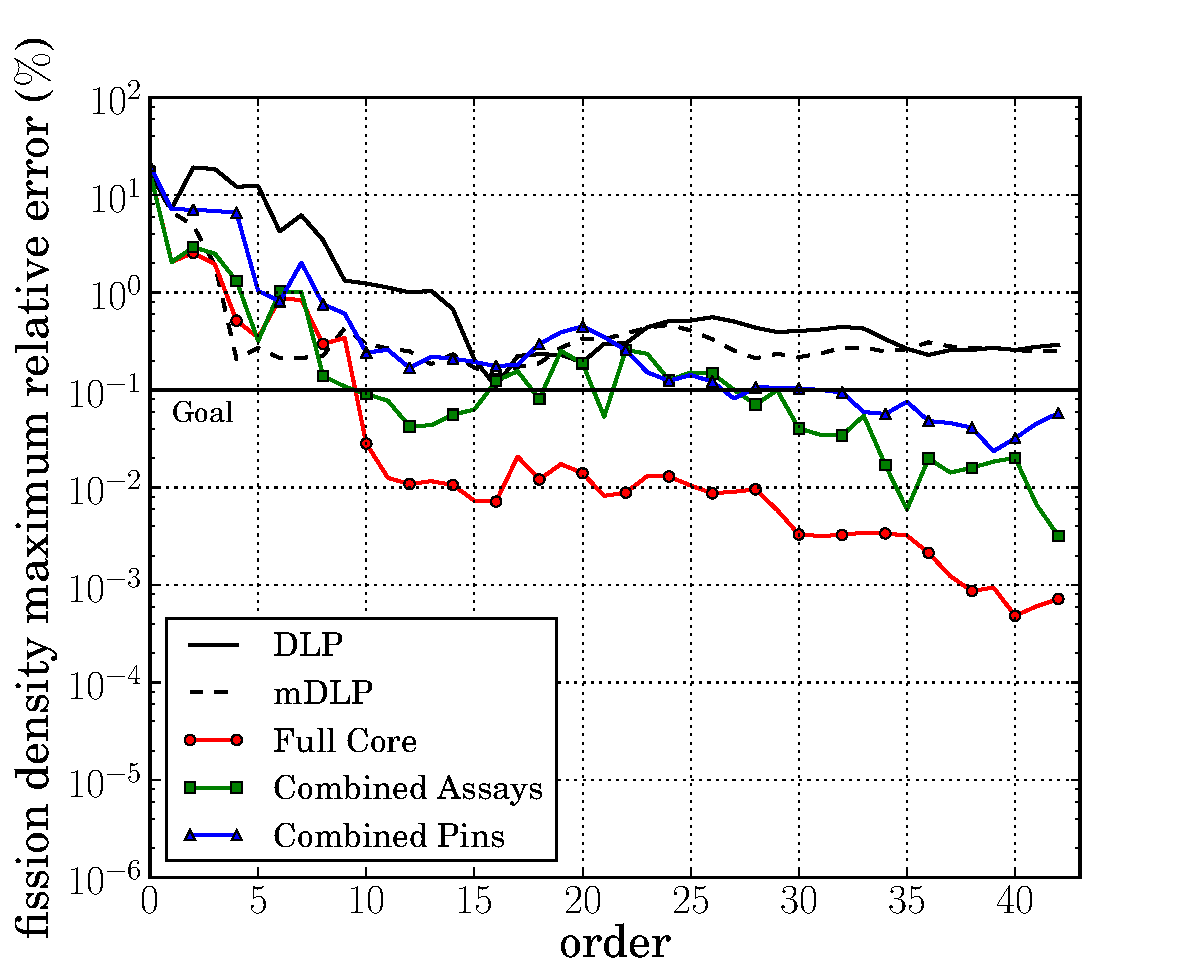
\includegraphics[trim=.1cm .25cm 2.0cm .4cm, clip=true,
            totalheight=0.261\textheight]
            {BWR2_238_partial_energy_basis_comparison_fission-44}
            \captionof{figure}{Using $\phi$ and $J_{\text{left}}$ data}
            \label{fig:core2-238b}
        \end{subfigure}
        \caption{Relative error for BWR test problem, Configuration 2, from
            238-group library}
        \label{fig:core2-238}
    \end{figure*}

    The practical models, combined-pins and combined-assemblies, required energy
    orders of approximately 25 and 15 when using only the scalar flux snapshots
    and using both scalar flux and partial current snapshots, respectively, for
    Configuration 0. In Configuration 1, the practical models required at
    least order 20 to reach the goal when using only scalar flux. Including
    snapshots of the partial current improved the results to 19th order.
    Configuration 2 required at least order
    30 when using only scalar flux snapshots, but dropped to approximately
    order 25 after
    including partial current snapshots.

    Despite the 238-group data containing substantially
    more detail in the energy spectra, the required orders for both test
    problems appeared roughly equivalent between the 44-group
    results and 238-group results. Thus, KLT can capture the finer details of
    energy dependent data in the low orders, thereby allowing for increased
    order reduction at a reduced accuracy penalty. This trend was expected to
    continue for other test problems that compared number of energy groups
    or for different, reasonably chosen group structures. Once
    again, the combined-pins model performed well in spite of the model
    simplicity, typically reaching the target accuracy at near the same order
as
    mDLP, despite requiring much less information {\it a priori}.

    Snapshots of the higher-order angular moments were then considered for the
    BWR test problem. All three configurations provided similar results, and
    the conclusion is identical to the 10-pin case, namely that including
    higher-order angular moments for basis generation did not
    yield any new information, meaning that the relative error derived from
    those snapshots was not significantly different from the partial current
snapshots.

    \subsection{Parametric Studies}

    To investigate KLT basis sets, several parametric studies were devised and
    explored. Two studies that warrant discussion are the sensitivity to
    the number
    of snapshots, and the second is the sensitivity
    to selection of snapshots. For the first study, the spatial
    discretization of the 10-pin test problem
    was varied to produce a greater or smaller number of
    spatial cells and potential snapshots. Results indicate that mesh size had
    a relatively
    small effect on the efficacy of the generated basis set. Additional
    snapshots taken from the same model are increasingly similar to the other
    snapshots, and thus do not add additional information to the expansion.

    In the second study, the effect of using a variable number of snapshots from
    the baseline BWR test problem was studied. The study used several snapshot
    selection schemes to select from the total snapshots. The first scheme was
    to use evenly spaced snapshots (i.e., only every $x$th snapshot was used to
    generate the basis). The second used a random selection of a given number.
    The third used
    the first $x$ snapshots, and the last scheme used $x$ snapshots from the
    center (because the problem was spatially symmetric). The resulting impact
    to fission density errors was negligible for the first two schemes, but the
    last two schemes produced a greater variation until snapshots from all types
    of cells were included. In other words, inclusion of additional snapshots
    does not affect the results unless the new snapshots are meaningfully
    distinct
    from the current set of snapshots. Based on these two studies, all
    available snapshots were used to produce figures in this paper. The error
    was not affected by the inclusion of additional, similar snapshots; only
    computation time was impacted, which was small compared to the application
    of ERMM.

    \section{Conclusions and Future Work}

    The KLT basis outperformed the mDLP and DLP bases for ERMM energy
    expansions
    because KLT, by construction, maximizes the amount of information contained
    in low-order expansions. When using appropriate data to generate the basis,
    sufficient accuracy (i.e., sub-$0.1\%$ maximum relative error in fission
    density) was obtained with as few as one-tenth of the equivalent energy
    degrees of freedom used in a full multigroup approximation. Smaller models
    used for snapshot generation provided encouraging results. In most cases,
    the KLT results based on small snapshot models were as good as or better
than those using mDLP despite requiring less
    information {\it a priori}. Furthermore, results were improved by including
    the partial
    current in snapshot generation.

    When solving test problems using different energy group structures (i.e.,
44-group
    and 238-group) with KLT bases, the resulting relative fission density
    errors were approximately the same, suggesting
    that efficiency of KLT is almost independent of the number of groups in the
    library. KLT can perform as well as or better relatively with the inclusion
of
    additional information from the higher group library compared to the lower
    group library. Because KLT is constructed to capture the most information
    in the low-order polynomials, and thus, the bases perform well no matter
    the number of groups.

    Results also suggested that adding more snapshots will improve the data only
    if the new snapshots are unique and representative of the problem space.
    Therefore, the inclusion of partial current snapshots improved results
    because the snapshots differed meaningfully from the scalar flux snapshots.
    Contrarily, the use of a greater number of snapshots from a finer spatial
    mesh yielded diminishing improvement because the new snapshots became
    increasingly similar. Most problems of interest contain a sufficiently
    large number of unique spatial regions for use in snapshot generation;
    therefore, a key goal of ongoing work is to determine other variables (e.g,
    increased angle dependence) that can provide greater snapshot variety.
    Additional ongoing work aims to extend the use of KLT energy expansions to
    2-D problems, for which the method is expected to yield similarly
    encouraging results.

    \section{Acknowledgements}
    The work of the first author was supported by the Kansas State University
Nuclear Research Fellowship Program, generously sponsored by the U.S. Nuclear
Regulatory Commission (Grant NRC-HQ-84-14-G-0033).

    \bibliographystyle{elsarticle-num}
    %\bibliographystyle{plainnat}
    \bibliography{bibliography}


\end{document}
